% Copyright (c) 2026 Jay Kerkar, Chaitanya Kelkar, Chirag Poornamath, Yash Kolekar and Shanta Sondur
% SPDX-License-Identifier: Apache-2.0
% SPIN 2027 (Springer LNEE proceedings), single-column llncs format. Wrapper only: the content is ../body.tex, the references
% are ../refs.bib, the figures and table macros are in figs/ (python -I paper/make_figs.py --width 4.803 --stack --out
% paper/springer/figs from the repository root: 122 mm wide, panels stacked, 8-9 pt text).
% Uses Springer's official llncs.cls v2.25 (2026/09/03) and splncs04.bst in this directory (checksums: ../vendor/*/provenance.json).
% Build: pdflatex main; bibtex main; pdflatex main; pdflatex main.
% Review build (anonymous) = the default. Camera-ready: change the next line to \anonymousfalse, or build with
%   pdflatex "\def\CAMERA{}% Copyright (c) 2026 Jay Kerkar, Chaitanya Kelkar, Chirag Poornamath, Yash Kolekar and Shanta Sondur
% SPDX-License-Identifier: Apache-2.0
% SPIN 2027 (Springer LNEE proceedings), single-column llncs format. Wrapper only: the content is ../body.tex, the references
% are ../refs.bib, the figures and table macros are in figs/ (python -I paper/make_figs.py --width 4.803 --stack --out
% paper/springer/figs from the repository root: 122 mm wide, panels stacked, 8-9 pt text).
% Uses Springer's official llncs.cls v2.25 (2026/09/03) and splncs04.bst in this directory (checksums: ../vendor/*/provenance.json).
% Build: pdflatex main; bibtex main; pdflatex main; pdflatex main.
% Review build (anonymous) = the default. Camera-ready: change the next line to \anonymousfalse, or build with
%   pdflatex "\def\CAMERA{}% Copyright (c) 2026 Jay Kerkar, Chaitanya Kelkar, Chirag Poornamath, Yash Kolekar and Shanta Sondur
% SPDX-License-Identifier: Apache-2.0
% SPIN 2027 (Springer LNEE proceedings), single-column llncs format. Wrapper only: the content is ../body.tex, the references
% are ../refs.bib, the figures and table macros are in figs/ (python -I paper/make_figs.py --width 4.803 --stack --out
% paper/springer/figs from the repository root: 122 mm wide, panels stacked, 8-9 pt text).
% Uses Springer's official llncs.cls v2.25 (2026/09/03) and splncs04.bst in this directory (checksums: ../vendor/*/provenance.json).
% Build: pdflatex main; bibtex main; pdflatex main; pdflatex main.
% Review build (anonymous) = the default. Camera-ready: change the next line to \anonymousfalse, or build with
%   pdflatex "\def\CAMERA{}% Copyright (c) 2026 Jay Kerkar, Chaitanya Kelkar, Chirag Poornamath, Yash Kolekar and Shanta Sondur
% SPDX-License-Identifier: Apache-2.0
% SPIN 2027 (Springer LNEE proceedings), single-column llncs format. Wrapper only: the content is ../body.tex, the references
% are ../refs.bib, the figures and table macros are in figs/ (python -I paper/make_figs.py --width 4.803 --stack --out
% paper/springer/figs from the repository root: 122 mm wide, panels stacked, 8-9 pt text).
% Uses Springer's official llncs.cls v2.25 (2026/09/03) and splncs04.bst in this directory (checksums: ../vendor/*/provenance.json).
% Build: pdflatex main; bibtex main; pdflatex main; pdflatex main.
% Review build (anonymous) = the default. Camera-ready: change the next line to \anonymousfalse, or build with
%   pdflatex "\def\CAMERA{}\input{main}".   \NOFV on the command line drops the formal-verification material.
\documentclass[runningheads]{llncs}
\newif\ifanonymous
\anonymoustrue   % <- the single switch: \anonymoustrue = review build, \anonymousfalse = camera-ready
\ifdefined\CAMERA\anonymousfalse\fi
\newif\iffv
\fvtrue
\ifdefined\NOFV\fvfalse\fi
\newif\ifshortpaper
\shortpapertrue
\newif\ifspringer
\springertrue
\newif\ifbibtexrefs
\bibtexrefstrue
\newcommand{\fpos}{!tb}
\renewcommand{\topfraction}{.85}\renewcommand{\bottomfraction}{.7}\renewcommand{\textfraction}{.1}\renewcommand{\floatpagefraction}{.7}                        % float placement: top or bottom of a page
\newcommand{\flowgap}{6.4cm}\newcommand{\flowtw}{5.3cm}   % Fig. 1 geometry (distance device-server, box text width)
\newcommand{\floatstart}[1]{\edef\floattmp{\noexpand\begin{#1}[\fpos]}\floattmp}   % \begin{#1}[placement]

\usepackage[T1]{fontenc}
\usepackage{amsmath,amssymb}
\usepackage{graphicx}
\usepackage{booktabs}
\usepackage{array}
\usepackage{textcomp}      % upright micro sign \textmu
\usepackage{url}
\usepackage{tikz}
\hfuzz=1pt                   % do not report sub-point overfull boxes
\setlength{\emergencystretch}{1em}   % only helps line breaking; no metric of the template changes
\usetikzlibrary{arrows.meta,positioning,calc}

% Cross-reference macros: "Sect. 7.5" (running text), "Section 7.5" (sentence start), "Fig. 2", "Table 2", "Eq. (1)".
% Pointers into the base paper are literal text in the body (e.g. "Table V of [1]") and do not use these.
\newcommand{\secref}[1]{Sect.~\ref{#1}}
\newcommand{\Secref}[1]{Section~\ref{#1}}
\newcommand{\secsref}[2]{Sects.~\ref{#1} and~\ref{#2}}
\newcommand{\figref}[1]{Fig.~\ref{#1}}
\newcommand{\tabref}[1]{Table~\ref{#1}}
\newcommand{\eqnref}[1]{Eq.~(\ref{#1})}
\newcommand{\designref}{Tables~\ref{tab:design} and~\ref{tab:designb}}
\newcommand{\runin}[1]{\paragraph{#1}}

% Keywords sit inside the abstract in llncs: 4-6 keywords, first letter capitalised.
\newcommand{\abstractkeywords}{%
\keywords{IoT authentication \and Pseudonym resolution \and Unlinkability \and Private identification \and Scalability%
\iffv \and ProVerif\fi}}
\newcommand{\afterabstract}{}

\begin{document}
\title{Pseudonym Resolution and Formal Verification of an Unlinkable Two-Message IoT Authentication Protocol}
\ifanonymous
  \titlerunning{Pseudonym Resolution in IoT Authentication}
  \author{Anonymous Author(s)}
  \authorrunning{Anonymous}
  \institute{Anonymous Institution}
  \pdfinfo{/Title (Pseudonym Resolution and Formal Verification of an Unlinkable Two-Message IoT Authentication Protocol) /Author ()}
\else
  \titlerunning{Pseudonym Resolution in IoT Authentication}
  \author{Jay Kerkar\inst{1}\orcidID{0009-0007-4612-6097} \and Chaitanya Kelkar\inst{1} \and Chirag Poornamath\inst{1} \and
  Yash Kolekar\inst{1} \and Shanta Sondur\inst{1}}
  \authorrunning{J. Kerkar et al.}
  \institute{Department of Information Technology, Vivekanand Education Society's Institute of Technology, Mumbai, India\\
  \email{jaykerkar0405@gmail.com, chaitanyakelkar07@gmail.com, chiragpoornamath@gmail.com, yashkolekar1234@gmail.com, shanta.sondur@ves.ac.in}}
  \pdfinfo{/Title (Pseudonym Resolution and Formal Verification of an Unlinkable Two-Message IoT Authentication Protocol) /Author (Jay Kerkar, Chaitanya Kelkar, Chirag Poornamath, Yash Kolekar, Shanta Sondur)}
\fi
\maketitle
\input{../body.tex}
\end{document}
".   \NOFV on the command line drops the formal-verification material.
\documentclass[runningheads]{llncs}
\newif\ifanonymous
\anonymoustrue   % <- the single switch: \anonymoustrue = review build, \anonymousfalse = camera-ready
\ifdefined\CAMERA\anonymousfalse\fi
\newif\iffv
\fvtrue
\ifdefined\NOFV\fvfalse\fi
\newif\ifshortpaper
\shortpapertrue
\newif\ifspringer
\springertrue
\newif\ifbibtexrefs
\bibtexrefstrue
\newcommand{\fpos}{!tb}
\renewcommand{\topfraction}{.85}\renewcommand{\bottomfraction}{.7}\renewcommand{\textfraction}{.1}\renewcommand{\floatpagefraction}{.7}                        % float placement: top or bottom of a page
\newcommand{\flowgap}{6.4cm}\newcommand{\flowtw}{5.3cm}   % Fig. 1 geometry (distance device-server, box text width)
\newcommand{\floatstart}[1]{\edef\floattmp{\noexpand\begin{#1}[\fpos]}\floattmp}   % \begin{#1}[placement]

\usepackage[T1]{fontenc}
\usepackage{amsmath,amssymb}
\usepackage{graphicx}
\usepackage{booktabs}
\usepackage{array}
\usepackage{textcomp}      % upright micro sign \textmu
\usepackage{url}
\usepackage{tikz}
\hfuzz=1pt                   % do not report sub-point overfull boxes
\setlength{\emergencystretch}{1em}   % only helps line breaking; no metric of the template changes
\usetikzlibrary{arrows.meta,positioning,calc}

% Cross-reference macros: "Sect. 7.5" (running text), "Section 7.5" (sentence start), "Fig. 2", "Table 2", "Eq. (1)".
% Pointers into the base paper are literal text in the body (e.g. "Table V of [1]") and do not use these.
\newcommand{\secref}[1]{Sect.~\ref{#1}}
\newcommand{\Secref}[1]{Section~\ref{#1}}
\newcommand{\secsref}[2]{Sects.~\ref{#1} and~\ref{#2}}
\newcommand{\figref}[1]{Fig.~\ref{#1}}
\newcommand{\tabref}[1]{Table~\ref{#1}}
\newcommand{\eqnref}[1]{Eq.~(\ref{#1})}
\newcommand{\designref}{Tables~\ref{tab:design} and~\ref{tab:designb}}
\newcommand{\runin}[1]{\paragraph{#1}}

% Keywords sit inside the abstract in llncs: 4-6 keywords, first letter capitalised.
\newcommand{\abstractkeywords}{%
\keywords{IoT authentication \and Pseudonym resolution \and Unlinkability \and Private identification \and Scalability%
\iffv \and ProVerif\fi}}
\newcommand{\afterabstract}{}

\begin{document}
\title{Pseudonym Resolution and Formal Verification of an Unlinkable Two-Message IoT Authentication Protocol}
\ifanonymous
  \titlerunning{Pseudonym Resolution in IoT Authentication}
  \author{Anonymous Author(s)}
  \authorrunning{Anonymous}
  \institute{Anonymous Institution}
  \pdfinfo{/Title (Pseudonym Resolution and Formal Verification of an Unlinkable Two-Message IoT Authentication Protocol) /Author ()}
\else
  \titlerunning{Pseudonym Resolution in IoT Authentication}
  \author{Jay Kerkar\inst{1}\orcidID{0009-0007-4612-6097} \and Chaitanya Kelkar\inst{1} \and Chirag Poornamath\inst{1} \and
  Yash Kolekar\inst{1} \and Shanta Sondur\inst{1}}
  \authorrunning{J. Kerkar et al.}
  \institute{Department of Information Technology, Vivekanand Education Society's Institute of Technology, Mumbai, India\\
  \email{jaykerkar0405@gmail.com, chaitanyakelkar07@gmail.com, chiragpoornamath@gmail.com, yashkolekar1234@gmail.com, shanta.sondur@ves.ac.in}}
  \pdfinfo{/Title (Pseudonym Resolution and Formal Verification of an Unlinkable Two-Message IoT Authentication Protocol) /Author (Jay Kerkar, Chaitanya Kelkar, Chirag Poornamath, Yash Kolekar, Shanta Sondur)}
\fi
\maketitle
% Copyright (c) 2026 Jay Kerkar, Chaitanya Kelkar, Chirag Poornamath, Yash Kolekar and Shanta Sondur
% SPDX-License-Identifier: Apache-2.0
% Shared body of all venue versions. \iffv ... \fi marks the material that only the version with formal verification contains.
% \ifanonymous (default false) removes everything that identifies the authors.
% Numbers come from figs/summary.json and figs/table_ranked.tex, written by make_figs.py.
%
% Contract with the wrapper (main.tex for IEEE, one wrapper per venue): before \input{body.tex} it defines
%   \iffv, \ifanonymous            switches
%   \ifspringer (single-column float layouts), \ifbibtexrefs (BibTeX list instead of the inline one), \runin, \Secref (sentence start), \designref, \abstractkeywords, \afterabstract (venue hooks)
%   \ifshortpaper (Springer page limit: drops the organisation paragraph, the complexity block of the ranked table and the "Specification gaps" paragraph)
%   \secref, \secsref, \figref, \tabref, \eqnref   venue-specific reference macros, e.g. \secref{x} -> "Section VII-E" (IEEE)
%                                  or "Sect. 7.5" (Springer). Pointers into the base paper are literal text and stay as they are.
% Springer camera-ready only (\ifbibtexrefs, not anonymous): the credits block before the references carries the funding,
% project-context and competing-interests statements supplied by the authors.
\newcommand{\PID}{\mathit{PID}}
\newcommand{\ID}{\mathit{ID}}
\newcommand{\Wc}{W_{\mathrm{c}}}
\input{figs/table_ranked.tex}

\begin{abstract}
Many lightweight IoT authentication protocols send an unlinkable pseudonym in clear and encrypt the rest under a
device-specific key, so the server must identify the sender before decrypting. We study this
resolution step for the two-message protocol of Al-Rasheed et al.\ (IEEE Transactions on Consumer Electronics, 2026), the
base paper. We show that every correct server needs the step, and that the base paper neither specifies nor costs it. We
implement the protocol, check it against independent reference vectors, and add seven resolution strategies: five that
keep the wire format, two that change the first message. Five adapt RFID privacy research. We measure probe counts and
price them with the base paper's constants in an OMNeT++ model of its network. Without resolution, our model
gives 23.86\,ms at one device, 0.8\% above the base paper's 23.68\,ms. At 1{,}000 devices with 5\%
adversaries, a precomputed table keeps the session at 24.4\,ms, while the on-demand scan reaches 44\,s, because each
forged pseudonym forces a full scan that no failure count sees. With counter epochs, a device that misses $F$
consecutive messages ($F=8$) is locked out for good. Varying our assumptions changes the absolute figures but not the
lead of the precomputed tables.
\iffv
ProVerif shows that session-key secrecy and agreement hold for every correct resolver, unlinkability holds with counter
epochs but fails with clock epochs, and injective device authentication needs replay state the specification leaves
open.
\fi
\ifanonymous
Code, models and data are open in the repository (link withheld for anonymous review).
\else
Code, models and data are open.
\fi
\abstractkeywords
\end{abstract}
\afterabstract


\section{Introduction}
Lightweight mutual-authentication protocols for IoT devices often hide the device's identity behind a pseudonym that
changes over time, so that an eavesdropper cannot link two sessions of the same device. Al-Rasheed et al.\ propose such a
protocol (IEEE Transactions on Consumer Electronics, 2026), which we call \emph{the base paper}~\cite{base}. Devices and
servers share pairwise keys from an offline phase, and they authenticate in two messages using symmetric primitives only;
the elliptic-curve operations from which the protocol takes its name belong to the offline phase. The device sends a
pseudonym $\PID=H_2(\lambda_V\|t)$, a hash of its long-term secret $\lambda_V$ and the epoch $t$, in clear. The epoch $t$
and the nonce $N_i$ travel inside a ciphertext under the pairwise key $k^\star$.

This design has a cost on the server side. The server cannot decrypt the first message until it knows which device sent
it, and the pseudonym is designed to hide exactly that. RFID privacy research has studied this tension for 20
years~\cite{weis,ohkubo,molnar,avoine05,ado05,tsudik}. It is known as \emph{private identification}: without
precomputation, a reader that must identify one of $n$ tags from an unlinkable response does $O(n)$ work. Recent RFID
work still aims at constant-time identification~\cite{tiplea}. In the base paper, the step is not specified, and its cost
model (Table~V and Eq.~22 of~\cite{base}) has no term for it. Its evaluation assigns the server a constant
$2T_H+2T_{SE/D}$ per session, whatever the number of devices; here $T_H=0.32$\,ms is the time of one hash and
$T_{SE/D}=5.6$\,ms the time of one symmetric encryption or decryption (Table~III of~\cite{base}).

\runin{Motivation.} Lightweight protocols are compared through the cost figures in their own evaluation tables. If a
step whose cost grows with the network is missing from those tables, the comparison favours the protocol for reasons that
do not survive deployment. We met this step while implementing the protocol: our first server had to scan every enrolled
device over a window of epochs for every incoming message, and that cost appears nowhere in~\cite{base}. An operator who
fills the step in the obvious way may therefore see sessions grow from milliseconds to seconds, or devices locked out,
with no warning from the published cost model.

\runin{Objective.} For the protocol of~\cite{base}, we set out to determine (i)~whether pseudonym resolution is required
and what the specification leaves open; (ii)~how the step can be filled, and what each choice costs in time and memory
as the network grows; (iii)~how each choice behaves under forged and dropped messages\iffv; and (iv)~which security
properties depend on the choice\fi. We answer these under the base paper's own constants and network, so that every result
can be compared directly with its published figures.

This paper makes the following contributions, which answer objective (i) (contribution~1), (ii) (2 and 3)\iffv, (iii)
(4) and (iv) (5)\else{} and (iii) (4)\fi:
\begin{enumerate}
\item \emph{The resolution gap.} From the specification alone, we show that every correct server must resolve the
pseudonym before any cryptographic check, and we state which choices the specification leaves open
(\secref{sec:gap}).
\item \emph{A design space.} We map seven strategies along the two open choices, the epoch semantics and the resolution
method: five that keep the wire format, and two that change the first message. Five of the seven adapt RFID work, and the
other two are ours. Each has a closed-form or measured cost (\secref{sec:design}).
\item \emph{A ranked comparison under the base paper's own conditions.} Probe counts measured on an open implementation
are priced with the constants of Table~III of~\cite{base}. They are evaluated in an OMNeT++ model of the network of
Table~II of~\cite{base}, and the one-device column is taken from the base paper itself. We also test how far the ranking
depends on our assumptions (\secref{sec:results}).
\item \emph{Failure modes.} We show the denial-of-service and desynchronisation behaviour of each strategy, including a
permanent lockout after $F$ dropped messages, which the threat model of the base paper allows
(\secsref{sec:probes}{sec:desync}).
\iffv
\item \emph{A formal analysis.} ProVerif models establish which security properties are independent of the resolver,
and which depend on the epoch and replay choices (\secref{sec:fv}).
\fi
\end{enumerate}

We do not re-evaluate the other results of~\cite{base}. We take its protocol as the specification and build on the parts
that we reproduced exactly.

\ifshortpaper\else
The rest of the paper is organised as follows. \Secref{sec:background} describes the protocol and the RFID work that we
adapt. \Secref{sec:gap} shows that resolution is required, and \secref{sec:design} defines the seven strategies.
\Secref{sec:method} describes the evaluation method, \secref{sec:validation} states how each result was validated, and
\secref{sec:results} gives the results.
\iffv
\Secref{sec:fv} presents the formal analysis.
\fi
\Secref{sec:disc} discusses the findings, \secref{sec:lim} lists the limitations, and \secref{sec:concl} concludes.
\fi

\section{Background}\label{sec:background}
\subsection{The Protocol}
In the offline phase, a trusted authority derives each entity's long-term secret $\lambda_X=H_1(\ID_X\|s)$ from the
entity's identifier $\ID_X$ and its master secret $s$. It gives each device--server pair the pairwise key
$k^\star=\mathrm{KDF}(\lambda_V\|\lambda_R)$, where KDF is a key derivation function (Eqs.~8--9 of~\cite{base}). Online,
in epoch $t$, the device $V$ samples $N_i$ and sends
\begin{equation*}
M_1=\langle\PID,\;\mathrm{AEAD}_{k^\star}(\PID\|N_i\|t)\rangle,\quad \PID=H_2(\lambda_V\|t).
\end{equation*}
AEAD is authenticated encryption with associated data; its authentication tag is the message authentication code
(MAC) $\mu_1$ of~\cite{base}. The server resolves $\PID$ to a device and an epoch, decrypts and verifies $M_1$, samples
$N_j$, and returns $M_2=\langle \ID_R,\mathrm{AEAD}_{k^\star}(N_j\|t;\,\PID\|N_i)\rangle$, where $\ID_R$ identifies the
server. Both sides derive $K=\mathrm{KDF}(k^\star\|N_i\|N_j\|t)$ (Eqs.~11--20 of~\cite{base}). We instantiate AEAD as
AES-256-GCM~\cite{gcm}, KDF as HKDF-SHA256 (HMAC-based KDF)~\cite{hkdf}, and both $H_1$ and $H_2$ as
SHA-256~\cite{fips180}, as the instantiation notes of~\cite{base} suggest. Our implementation adds no domain-separation
tag: $H_1$ hashes the identifier and the master secret, and $H_2$ hashes the 32-byte $\lambda$ and the epoch as an 8-byte
big-endian integer.

We implemented this exchange in Python, with a C port of the device side, and validated both against independent
reference vectors (\secref{sec:validation}). The vectors fix the message layout that the next section relies on: the
pseudonym is the only field in clear, and $N_i$ and $t$ are inside the AEAD ciphertext under $k^\star$.

\subsection{Private Identification in RFID}
The same problem appears when an RFID reader must identify a tag that answers with an unlinkable value. Five lines of work
define the strategies we adapt:
\begin{itemize}
\item \emph{Randomised hash lock}~\cite{weis}: the tag answers $(r, H(k\|r))$ for a fresh $r$, and the reader tries every
key, $O(n)$.
\item \emph{Hash chains} (OSK, after Ohkubo, Suzuki and Kinoshita)~\cite{ohkubo}: the tag's state evolves by a one-way
function, which gives forward privacy. The reader searches $n$ chains up to depth $m$, $O(nm)$. Our counter epochs are the
same search with the chain replaced by $H_2(\lambda\|t)$.
\item \emph{Key trees}~\cite{molnar}: keys form a tree of branching factor $\delta$, and the tag answers with one keyed
hash per level, $O(\delta\log_\delta n)$. Tags share their internal keys, so compromising one tag weakens the privacy of
others~\cite{ado05}.
\item \emph{Time-memory trade-off}~\cite{avoine05,ado05}: Hellman-style~\cite{hellman} rainbow tables~\cite{oechslin}
over all $(\text{tag},\ \text{state})$ pairs bring OSK to $O((nm)^{2/3})$ time and memory.
\item \emph{Time-based pseudonyms}, as in YA-TRAP~\cite{tsudik}: the reader precomputes one table per time period.
\end{itemize}

\ifshortpaper\else
Avoine et al.~\cite{ado05} compared these approaches by time and memory for one tag. \Secref{sec:results} makes the same
comparison for this protocol, at network scale and under the base paper's own constants.
\fi

\section{The Resolution Gap}\label{sec:gap}
\ifshortpaper\else
Each step of the argument uses only the specification, or a fact that our reference vectors confirm.
\fi
\begin{enumerate}
\item $M_1$ carries $\PID$ in clear. The epoch $t$ and nonce $N_i$ are only inside the ciphertext under $k^\star$
(Eqs.~13--15 of~\cite{base}; confirmed byte for byte).
\item $k^\star=\mathrm{KDF}(\lambda_V\|\lambda_R)$ is specific to the device (Eqs.~9 and 12 of~\cite{base}).
\item So the server cannot decrypt $M_1$ or verify its tag $\mu_1$ until it knows which device sent it.
\item The base paper requires that $\PID$ cannot be linked to $V$ without $\lambda_V$ (Section~III-J of~\cite{base}). So
the device's identity cannot be read from $M_1$ either.
\item So every correct server must map $\PID$ to $(V,t)$ by computing pseudonyms from the secrets it holds. We call this
step \emph{pseudonym resolution} (\figref{fig:flow}).
\end{enumerate}

The specification says only that the pseudonym is ``rotated with time (or epoch) $t$''. It leaves two choices open, and
together they decide the cost:
\begin{itemize}
\item \emph{Epoch semantics}: a per-device counter, or a clock.
\item \emph{Resolution method}: an on-demand search, or a table prepared in advance.
\end{itemize}

Table~V of~\cite{base} charges the server $2T_H+2T_{SE/D}$ per session, and Eq.~22 of~\cite{base} lists a fixed number of
KDF, encryption, decryption and MAC operations. Neither contains a term that grows with the number of devices. We count
resolution cost in \emph{probes}, where one probe is one evaluation of $H_2$ (or the equivalent keyed hash), and price it
at $T_H$ from Table~III of~\cite{base}. Throughout, $n$ is the number of devices enrolled at one server and $N$ the number
of devices in the network.

\floatstart{figure}
\centering
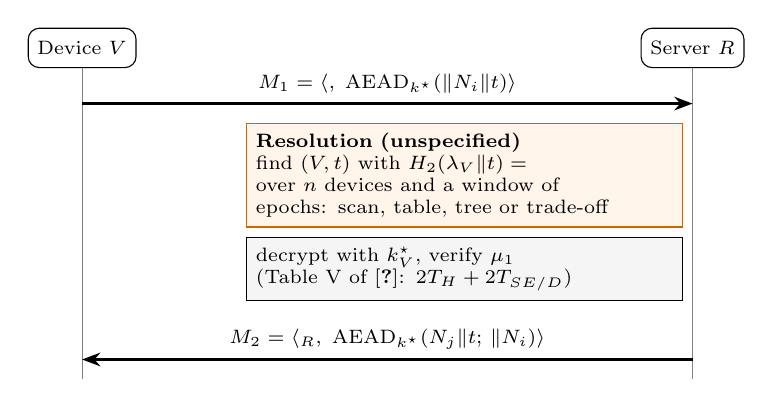
\begin{tikzpicture}[font=\scriptsize, >=Stealth, node distance=4mm]
\node[draw, rounded corners, minimum width=1.3cm, minimum height=5mm] (D) {Device $V$};
\node[draw, rounded corners, minimum width=1.3cm, minimum height=5mm, right=\flowgap of D] (S) {Server $R$};
\draw[gray] (D.south) -- ++(0,-3.95);
\draw[gray] (S.south) -- ++(0,-3.95);
\draw[->, thick] ($(D.south)+(0,-0.45)$) -- node[above, align=center]{$M_1=\langle \PID,\;\mathrm{AEAD}_{k^\star}(\PID\|N_i\|t)\rangle$} ($(S.south)+(0,-0.45)$);
\node[draw=orange!80!black, fill=orange!8, align=left, anchor=north east, text width=\flowtw] (R) at ($(S.south)+(-0.12,-0.7)$)
 {\textbf{Resolution (unspecified)}\\ find $(V,t)$ with $H_2(\lambda_V\|t)=\PID$\\ over $n$ devices and a window of\\ epochs: scan, table, tree or trade-off};
\node[draw, fill=gray!8, align=left, anchor=north east, text width=\flowtw] (V) at ($(R.south east)+(0,-0.12)$)
 {decrypt with $k^\star_V$, verify $\mu_1$\\ (Table~V of~\cite{base}: $2T_H+2T_{SE/D}$)};
\draw[<-, thick] ($(D.south)+(0,-3.7)$) -- node[above]{$M_2=\langle \ID_R,\;\mathrm{AEAD}_{k^\star}(N_j\|t;\,\PID\|N_i)\rangle$} ($(S.south)+(0,-3.7)$);
\end{tikzpicture}
\caption{Position of pseudonym resolution in the exchange. The server needs $k^\star_V$ to open $M_1$, but $V$ is hidden behind $\PID$.}
\label{fig:flow}
\end{figure}

\section{Design Space}\label{sec:design}
We implemented seven strategies (\designref), which we label O1 to O4, TM, CR and MW. The first five keep the wire
format of $M_1$. The last two need a fresh $r$ in clear, so they change $M_1$. They are modelled at the resolution level,
with the same keyed hash.
\begin{itemize}
\item \textbf{O1}, counter with a linear scan, is the behaviour of our original implementation. For each device it probes
epochs $\ell-L$ to $\ell+F$, where $\ell$ is the last accepted epoch, $L=16$ is the number of epochs below $\ell$ that the
server still checks (the replay lookback) and $F=8$ the number of epochs above it (the forward tolerance). The window is
$W=L+F+1=25$ epochs.
\item \textbf{O2} keeps a table of every device's next $F$ pseudonyms and slides it after each acceptance.
\item \textbf{O3} and \textbf{O4} use clock epochs with a drift window $\Wc=3$ (the current epoch and one on each side).
O3 scans, and O4 extends a table once per epoch.
\item \textbf{TM}, the time-memory trade-off, is a rainbow table over $S=nm$ points, with lifetime $m=128$ epochs per
device, chain length $S^{1/3}$ rounded to the nearest integer, $2S^{2/3}$ chains per table, and six tables.
\item \textbf{CR}, the challenge-response randomised hash lock, adds a fresh 128-bit $r$ to $M_1$ and tries every enrolled
key in turn. It keeps no resolution state and has no epochs.
\item \textbf{MW}, the key tree of Molnar and Wagner, uses branching factor $\delta=32$ and depth $d$, the number of tree
levels. For $n\le1{,}024$ the tree has $d\le2$ levels. The device adds $r$ and $d-1$ tags to $M_1$.
\end{itemize}

\ifspringer
\floatstart{table}
\centering
\caption{Design space, cost. $n$: devices enrolled at the server; $L=16$, $F=8$, $W=L+F+1$; $\Wc=3$; $S=nm$; $d$: depth of the
MW tree. ``Probes'' are expected $H_2$ evaluations per message, in steady state.}
\label{tab:design}
\footnotesize
\setlength{\tabcolsep}{2pt}
\begin{tabular}{@{}l l p{2.7cm} p{2.3cm} l@{}}
\toprule
Strategy & Epoch / $M_1$ & Probes, honest & Probes, forged & Precompute \\
\midrule
O1 & counter / unchanged & $\frac{(n-1)W}{2}+L+2$ & $nW$ & none \\
O2 & counter / unchanged & $1$ (slide) & $0$ & $nF$ once \\
O3 & clock / unchanged & $\frac{(n-1)\Wc}{2}+1$ & $n\Wc$ & none \\
O4 & clock / unchanged & $0$ & $0$ & $n$ per epoch \\
TM & counter / unchanged & $\approx0.5$--$0.7\,S^{2/3}$ (meas.) & $\approx4\,S^{2/3}$ (meas.) & $\approx12S$ once \\
CR & none / $+r$ (128 bits) & $\frac{n+1}{2}$ & $n$ & none \\
MW & none / $+r$, $+(d-1)$ tags & $\le\delta d$ & $\le\delta$ & none \\
\bottomrule
\end{tabular}
\end{table}

\floatstart{table}
\centering
\caption{Design space, state and behaviour (same strategies as Table~\ref{tab:design}). One table entry is 40 bytes and one
nonce-cache entry 24 bytes.}
\label{tab:designb}
\footnotesize
\setlength{\tabcolsep}{3pt}
\begin{tabular}{@{}l l l l@{}}
\toprule
Strategy & Resolution state & Dropped $M_1$ & Linkability \\
\midrule
O1 & $8n$ bytes & lockout after $F$ & none \\
O2 & $(40F+8)n$ bytes & lockout after $F$ & none \\
O3 & $24n$ bytes (nonce cache) & none & same epoch \\
O4 & $(40\Wc+24)n$ bytes & none & same epoch \\
TM & $\approx50\,S^{2/3}$ bytes & none until $t=m$ & none \\
CR & none & none & none \\
MW & 32 bytes per internal node & none & after compromise \\
\bottomrule
\end{tabular}
\end{table}
\else
\floatstart{table*}
\centering
\caption{Design space. $n$: devices enrolled at the server; $L=16$, $F=8$, $W=L+F+1$; $\Wc=3$; $S=nm$; $d$: depth of the
MW tree. One table entry is 40 bytes and one nonce-cache entry 24 bytes. ``Probes'' are expected $H_2$ evaluations per
message, in steady state.}
\label{tab:design}
\footnotesize
\setlength{\tabcolsep}{2.4pt}
\begin{tabular}{@{}l l l l l l l l@{}}
\toprule
Strategy & Epoch / $M_1$ & Probes, honest & Probes, forged & Precompute & Resolution state & Dropped $M_1$ & Linkability \\
\midrule
O1 & counter / unchanged & $\frac{(n-1)W}{2}+L+2$ & $nW$ & none & $8n$ bytes & lockout after $F$ & none \\
O2 & counter / unchanged & $1$ (slide) & $0$ & $nF$ once & $(40F+8)n$ bytes & lockout after $F$ & none \\
O3 & clock / unchanged & $\frac{(n-1)\Wc}{2}+1$ & $n\Wc$ & none & $24n$ bytes (nonce cache) & none & same epoch \\
O4 & clock / unchanged & $0$ & $0$ & $n$ per epoch & $(40\Wc+24)n$ bytes & none & same epoch \\
TM & counter / unchanged & $\approx0.5$--$0.7\,S^{2/3}$ (meas.) & $\approx4\,S^{2/3}$ (meas.) & $\approx12S$ once & $\approx50\,S^{2/3}$ bytes & none until $t=m$ & none \\
CR & none / $+r$ (128 bits) & $\frac{n+1}{2}$ & $n$ & none & none & none & none \\
MW & none / $+r$, $+(d-1)$ tags & $\le\delta d$ & $\le\delta$ & none & 32 bytes per internal node & none & after compromise \\
\bottomrule
\end{tabular}
\end{table*}
\fi

\section{Evaluation Method}\label{sec:method}
We follow the base paper's evaluation conditions and change only the resolution term.
\begin{itemize}
\item \emph{Simulator and environment}: OMNeT++ 6.4~\cite{omnet} (Cmdenv), with Table~II of~\cite{base}: a
1{,}500\,m $\times$ 1{,}500\,m area, 10\,Mb/s, 500\,m range, 75.6\,mW, a 15\,\textmu s quantum, servers at 5\% of the devices.
\item \emph{Protocol cost}: Tables~III--V of~\cite{base}. That is $2T_H+2T_{SE/D}=11.84$\,ms per side, $T_H=0.32$\,ms per
probe, and 1{,}024 bits, which Table~IV of~\cite{base} lists for four messages although the protocol has two.
\item \emph{Resolution cost}: for each server we look up the probes for its number of enrolled devices $n$ in the
measured cost model. It is exact for O1--O4 and CR, and interpolated between measured points for TM and MW. CR and MW
also add their extra $M_1$ bits. At $N\ge100$ each server enrols about a quarter of the devices ($n\approx258$ at
$N=1{,}000$).
\item \emph{Assumptions} (the base paper does not fix these): an adversary share of 5\%, each sending forged $M_1$ at
1\,Hz; a 10\,s window in which each device starts one authentication; \emph{reachable enrolment}, in which each server
enrols every device in its radio range (the alternative, \emph{nearest enrolment}, enrols each device only at the server
nearest to it); first-come-first-served server processing; for O4, one epoch extension per server inside the window.
\item \emph{Runs}: five seeds per point, at 12 network sizes ($N=1$, 10, 100, and 200 to 1{,}000 in steps of 100), and eight
configurations: the seven strategies and, as the eighth, the baseline without resolution. Each is run with and without
adversaries. That is $12\times8\times5\times2=960$ runs, reported as means.
\end{itemize}

The model is ours, not the authors' (\secref{sec:validation} gives its validation, and \secref{sec:sens} the effect of
these assumptions). The base column of \tabref{tab:ranked} ($N=1$) is therefore the base paper's own figure: 23.68\,ms from
Tables~III and~V of~\cite{base}, and 320 bits (40 bytes) of server storage from Table~VI of~\cite{base}. Latency in \tabref{tab:ranked}
is the mean per-session latency over five seeds. Storage at larger $N$ is those 320 bits per enrolled device plus the
resolution state, averaged over the servers of the simulated network; 1\,KiB is 1{,}024 bytes throughout.

\section{Validation}\label{sec:validation}
Each result rests on one of these checks, all of which can be rerun from the repository.
\begin{itemize}
\item \emph{Protocol implementation.} The Python implementation and the C port of the device side reproduce reference
vectors byte for byte (15 checks each). The vectors were computed by a generator that shares no code with either
implementation. They cover the pairwise key, the pseudonym, the wire bytes of $M_1$ and $M_2$, and the session key,
together with the rejection of tampered and replayed messages. A C device and the Python server complete five handshakes
with matching session keys, and the server rejects a replayed $M_1$. All 125 unit and property tests pass.
\item \emph{Resolution strategies.} For each strategy and each
$n\in\{$1, 2, 5, 10, 20, 50, 100, 200, 300, 500, 700, 1{,}000, 2{,}000, 5{,}000, 10{,}000$\}$ (15 values), a script builds the server in
steady state. It resolves 200 pseudonyms of randomly drawn devices (50 for O1, O3, TM and CR above $n=2{,}000$) and five
forged ones, and counts every $H_2$ call. For O1--O4 and CR, the forged and per-epoch counts and the state equal the closed
forms of \designref exactly. O2 and O4 need exactly 1 and 0 probes per authentication. The honest means of O1, O3
and CR lie within four standard errors of the formulas, and MW never exceeds $\delta d$. In our parameter runs ($n=40$ to
500), the TM tables covered 99.6--99.8\% of points. In the sweep, they missed 9 of 2{,}100 honest pseudonyms, the samples
at the 12 sizes with $n\ge10$ (10 sizes with 200 pseudonyms and 2 with 50); the device then retries with its next epoch.
A total of 12 unit tests run each wire-compatible strategy through the full handshake and check its probe counts, replay rejection and
lockout. A rerun of the sweep reproduced every non-TM count exactly; TM varies because its peer secrets are random.
\item \emph{Network model.} With the resolution term removed, the model gives 23.86\,ms at $N=1$ and 24.07\,ms at
$N=1{,}000$, against the base paper's arithmetic value of 23.68\,ms. The 0.8--1.7\% difference is airtime and
quantisation, which the arithmetic leaves out. In the baseline row of \tabref{tab:sens}, the load of the mean server,
computed independently of the simulator from the cost model, orders the strategies exactly as the simulation does
(\secref{sec:sens}).
\iffv
\ifshortpaper\else
\item \emph{Security properties.} ProVerif checks the security claims symbolically (\secref{sec:fv}).
\fi
\fi
\end{itemize}

\runin{Limits of the validation.} The code of the base paper is not available, so the vectors encode our reading of
Section~III of~\cite{base}: both implementations agree with that reading, which may not be what its authors intended. The
network model is checked against the base paper only at one device without resolution, the one point where it gives a
figure, and its saturated behaviour has not been compared with another simulator.

\section{Results}\label{sec:results}
\ifspringer
\floatstart{table}
\centering
\caption{Strategies ranked from best to worst by mean session latency at $N=1{,}000$ (5\% adversaries), in the OMNeT++
model of the network of Table~II of~\cite{base} with the constants of its Table~III (\secref{sec:method}). Storage: mean per
server. The base column ($N=1$) is the value published in~\cite{base}: 23.68\,ms and 320 bits.}
\label{tab:ranked}
\footnotesize
\setlength{\tabcolsep}{2pt}
\ifshortpaper
\begin{tabular}{@{}c l r r r r r@{\hspace{9pt}}r r r r r@{}}
\toprule
 & & \multicolumn{5}{c}{Mean session latency (ms), by $N$} & \multicolumn{5}{c}{Storage per server (KiB), by $N$} \\
\cmidrule(lr){3-7}\cmidrule(l){8-12}
\# & Strategy & base & 10 & 100 & 500 & 1{,}000 & base & 10 & 100 & 500 & 1{,}000 \\
\midrule
\rankedlsrows
\bottomrule
\end{tabular}
\else
\begin{tabular}{@{}c l l l@{}}
\toprule
\# & Strategy & Time per auth. & Space per auth. \\
\midrule
\rankedcomprows
\bottomrule
\end{tabular}

\medskip
\begin{tabular}{@{}c l r r r r r@{}}
\toprule
 & & \multicolumn{5}{c}{Mean session latency (ms), by $N$} \\
\cmidrule(l){3-7}
\# & Strategy & base & 10 & 100 & 500 & 1{,}000 \\
\midrule
\rankedlatrows
\bottomrule
\end{tabular}

\medskip
\begin{tabular}{@{}c l r r r r r@{}}
\toprule
 & & \multicolumn{5}{c}{Storage per server (KiB), by $N$} \\
\cmidrule(l){3-7}
\# & Strategy & base & 10 & 100 & 500 & 1{,}000 \\
\midrule
\rankedstorrows
\bottomrule
\end{tabular}
\fi
\end{table}
\else
\floatstart{table*}
\centering
\caption{Strategies ranked from best to worst by mean session latency at $N=1{,}000$ (5\% adversaries), in the OMNeT++
model of the network of Table~II of~\cite{base} with the constants of its Table~III (\secref{sec:method}). Storage: mean per
server. The base column ($N=1$) is the value published in~\cite{base}: 23.68\,ms and 320 bits.}
\label{tab:ranked}
\footnotesize
\setlength{\tabcolsep}{2pt}
\begin{tabular}{@{}c l l l l r r r r r r r r r r@{}}
\toprule
 & & & \multicolumn{2}{c}{Complexity per auth.} & \multicolumn{5}{c}{Mean session latency (ms), by $N$} & \multicolumn{5}{c}{Storage per server (KiB), by $N$} \\
\cmidrule(lr){4-5}\cmidrule(lr){6-10}\cmidrule(l){11-15}
\# & & Strategy & Time & Space & base & 10 & 100 & 500 & 1{,}000 & base & 10 & 100 & 500 & 1{,}000 \\
\midrule
\rankedrows
\bottomrule
\end{tabular}
\end{table*}
\fi

\floatstart{figure*}
\centering
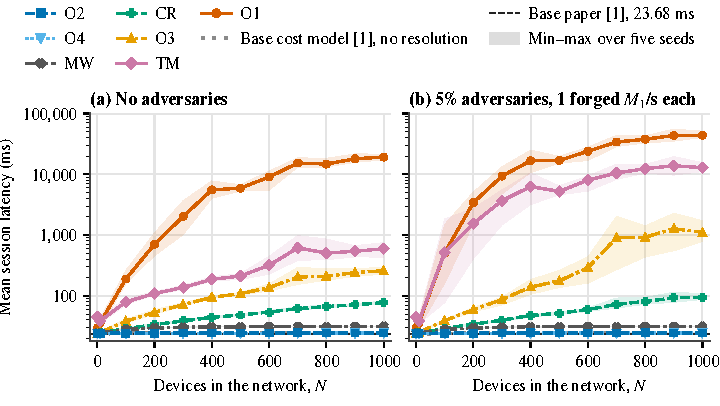
\includegraphics[width=\textwidth]{figs/fig_latency.pdf}
\caption{Mean session latency against network size in the OMNeT++ model (log scale; band: minimum to maximum over five
seeds). (a) Without adversaries. (b) With 5\% adversaries, each sending one forged $M_1$ per second. Dotted: the cost model of~\cite{base} with no resolution. Dashed: the base paper's 23.68\,ms.}
\label{fig:latency}
\end{figure*}

\subsection{Ranking}
\tabref{tab:ranked} gives the ranking. The two table strategies, O2 and O4, stay within 1\,ms of the base paper's figure up
to 1{,}000 devices. O2 needs one probe to slide the window, and O4 only the per-epoch extension. Their cost is memory: at
1{,}000 devices, about 93\,KiB and 46\,KiB per server, against 10\,KiB for Table~VI of~\cite{base} alone. The key tree is
third (31.4\,ms). It changes $M_1$, and a compromised device leaks the internal keys it shares with others. The
randomised hash lock (CR) needs no extra state, but its latency grows linearly, to 95\,ms. The three scanning strategies
with epochs saturate the server: clock scan (O3) at 1.1\,s, the time-memory trade-off at 12.9\,s, and the counter scan
(O1) at 44\,s. For O1 and TM, the spread across seeds at $N=1{,}000$ is 10.6\,s and 4.5\,s, because the latency depends on
how many devices and adversaries share the busiest server.

\subsection{Honest Load Against Forged Load}\label{sec:probes}
\figref{fig:latency} separates the two causes. Without adversaries (a), O1 already reaches 19.2\,s at 1{,}000 devices.
Each honest authentication costs about $12.5\,n$ probes, which is 1.0\,s of hashing at the $n\approx258$ devices that a
server enrols at $N=1{,}000$ ($T_H=0.32$\,ms). Arrivals outpace this, so the server queue grows. The forged load (b)
roughly doubles this, because every forged pseudonym costs a full miss scan of $Wn$ probes. Such a pseudonym never resolves
to a device, so the block-list, which blocks a device after three consecutive failed attempts, never sees it.
\figref{fig:probes} shows the same effect for one server enrolling up to $n=10{,}000$ devices. A forgery costs O1 250,000
probes and TM about 46,000, but costs O2 and O4 nothing, because a table miss needs no hash.

\floatstart{figure*}
\centering
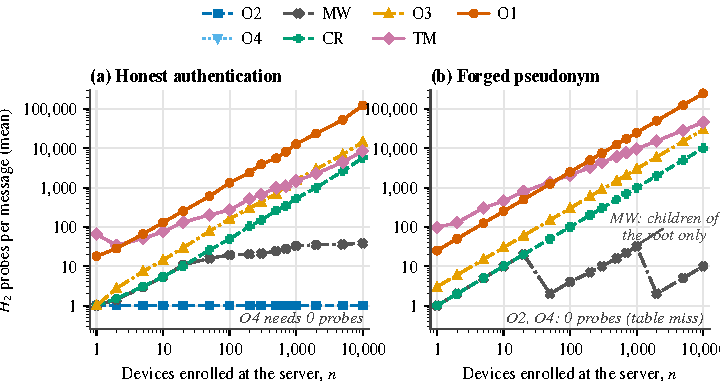
\includegraphics[width=\textwidth]{figs/fig_probes.pdf}
\caption{Probes per message at one server, measured on the implementation (log-log). (a) Honest authentication. (b) A
forged, random pseudonym.}
\label{fig:probes}
\end{figure*}

\subsection{Time Against Memory}
\figref{fig:storage} shows storage at one server, and each strategy's position in the time-memory plane for one server
enrolling $n=1{,}000$ devices. Storage is the resolution state plus the 40 bytes (320 bits) per device of Table~VI
of~\cite{base}. No strategy that keeps the wire format is both fast and small. O2 buys constant time with $F$ table entries
per device (359\,KiB in total), and O4 with $\Wc$ entries per device (180\,KiB). TM sits in between, at 167\,KiB and 1{,}478
probes. It is dominated here because its table must cover the device's whole lifetime ($m=128$ epochs), not just the
current window. MW is the only point that is both small and fast, and it pays with a different $M_1$ and a weaker privacy
model.

\floatstart{figure*}
\centering
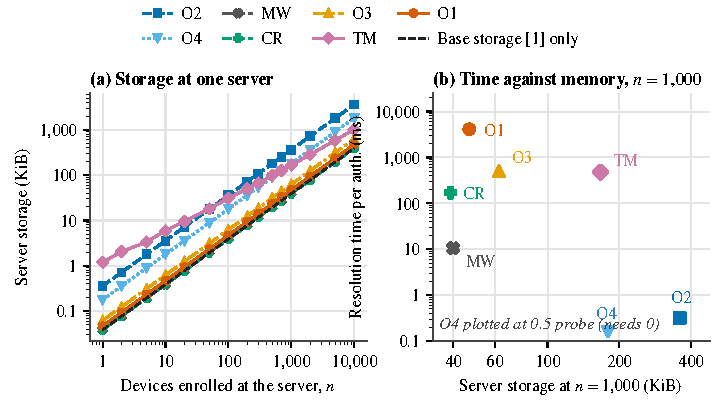
\includegraphics[width=\textwidth]{figs/fig_storage.pdf}
\caption{(a) Server storage (the 320 bits per device of Table~VI of~\cite{base} plus the resolution state) for one server.
(b) Resolution time per authentication ($T_H=0.32$\,ms per probe) against storage, for one server enrolling 1{,}000
devices.}
\label{fig:storage}
\end{figure*}

\subsection{Desynchronisation}\label{sec:desync}
With counter epochs, the device advances $t$ every time it builds $M_1$. The server searches at most $F$ epochs ahead of
the last one it accepted. In our implementation, an adversary who drops $F=8$ consecutive $M_1$ messages locks the device
out for good: every later handshake fails with an unknown pseudonym, with or without an earlier successful session. The
lockout holds for O1 and O2, and a unit test checks it for both. The threshold is $F$, which the specification does not
fix. A larger $F$ delays the lockout but does not remove it. A device whose counter lives in RAM is also rejected as
a replay after a restart; we observed this for O1. Message dropping is within the threat model of~\cite{base}. Clock epochs
(O3, O4), CR and MW have no per-device counter, so they cannot desynchronise this way. TM tolerates any number of drops
until $t$ reaches the lifetime $m$.

\subsection{Sensitivity to the Assumptions}\label{sec:sens}
The base paper does not fix the adversary share and rate, the authentication window or the enrolment rule, and $T_H$ is its
constant, not our measurement. We bound their effect without new simulation runs. First, the simulation was run with and
without adversaries (\figref{fig:latency}): at $N=1{,}000$ the ranking is the same, and O2, O4 and MW move by less than
0.2\,ms. Second, we compute the offered load of the mean server at $N=1{,}000$ from the committed cost model,
$\rho=\alpha_h(C_R+hT_H)+\alpha_a fT_H$, where $C_R=11.84$\,ms is the server cost per session from Tables~III and~V of~\cite{base},
$h$ and $f$ are the measured honest and forged probes at the mean enrolment $n=258$, and $\alpha_h$ and $\alpha_a$ are the
honest and forged arrival rates per server. $\rho\ge1$ means saturation (\tabref{tab:sens}).

\floatstart{table}
\centering
\caption{Offered load $\rho$ of the mean server at $N=1{,}000$, one assumption varied at a time from the baseline (5\%
adversaries at 1\,Hz, 10\,s window, reachable enrolment, $T_H=0.32$\,ms). $\rho\ge1$: saturated.}
\label{tab:sens}
\footnotesize
\setlength{\tabcolsep}{2.6pt}
\begin{tabular}{@{}l r r r r r r r@{}}
\toprule
Case & O2 & O4 & MW & CR & O3 & TM & O1 \\
\midrule
Baseline              & 0.02 & 0.03 & 0.04 & 0.19 & 0.52 & 1.68 & 4.16 \\
No adversaries        & 0.02 & 0.03 & 0.04 & 0.11 & 0.27 & 0.41 & 2.09 \\
20\% adversaries      & 0.02 & 0.03 & 0.05 & 0.44 & 1.26 & 5.47 & 10.3 \\
Adversary rate 2\,Hz  & 0.02 & 0.03 & 0.04 & 0.27 & 0.77 & 2.94 & 6.22 \\
Window 5\,s           & 0.05 & 0.06 & 0.08 & 0.30 & 0.79 & 2.09 & 6.25 \\
Window 20\,s          & 0.01 & 0.02 & 0.02 & 0.14 & 0.38 & 1.47 & 3.11 \\
$T_H=0.16$\,ms        & 0.02 & 0.03 & 0.03 & 0.11 & 0.27 & 0.85 & 2.09 \\
$T_H=0.64$\,ms        & 0.03 & 0.04 & 0.06 & 0.36 & 1.01 & 3.33 & 8.29 \\
Nearest enrolment     & 0.02 & 0.02 & 0.04 & 0.04 & 0.06 & 0.36 & 0.35 \\
\bottomrule
\end{tabular}
\end{table}

Except in the last row, the order by $\rho$ is that of \tabref{tab:ranked}, and O2 and O4 do not exceed 0.06. The
absolute figures do depend on the assumptions: O1 saturates unless $T_H<0.076$\,ms, and O3 saturates with 20\%
adversaries or $T_H=0.64$\,ms. (The busiest server enrols up to 396 devices, which is why O3 already queues in the
simulation at $\rho=0.52$.) If a server enrols only the devices attached to it ($n\approx20$), nothing saturates and the
lower ranks reorder, but O2 and O4 stay first. $L$, $F$ and $\Wc$ act only through the closed forms of
\designref. The recommendation of \secref{sec:disc} therefore holds under every assumption we varied, while
figures such as O1's 44\,s hold only under the baseline.

\iffv
\section{Formal Verification}\label{sec:fv}
We modelled the exchange in ProVerif~2.05~\cite{proverif}, in the symbolic model with an active attacker
(\tabref{tab:fv}). Other lightweight IoT schemes are checked in the same tool~\cite{wu22,lee25}; the scheme of~\cite{lee25},
for example, proves the privacy of its pseudonyms in ProVerif~2.05. Our hash, KDF and AEAD are free functions, and AEAD has
associated data. The main model has unbounded servers, unbounded honest and corrupt devices per server, and unbounded
sessions. A corrupt device's $\lambda$ and $k^\star$ are given to the attacker. The server may resolve a pseudonym to
\emph{any} enrolled device, and must then decrypt and check $\PID=H_2(\lambda_V\|t)$. So every result that holds, holds for
every resolver that returns a correct device. Epochs are fresh values, and the server keeps no replay state. Unlinkability
is checked as observational equivalence~\cite{blanchet08}, in the style of~\cite{arapinis}: one device running twice,
against two devices running once each. On both sides the server knows both devices and resolves with one destructor.

\floatstart{table}
\centering
\caption{ProVerif results (all models finish in under 1\,s).}
\label{tab:fv}
\footnotesize
\begin{tabular}{@{}l p{3.6cm} p{2.6cm}@{}}
\toprule
Query & Property & Result \\
\midrule
Q1, Q2 & Session key secret (device and server side) & holds \\
Q3 & Server accepts $M_1$ of honest $V$ $\Rightarrow$ $V$ sent it & holds \\
Q4 & Same, injective & fails (replay, no replay state) \\
Q5 & Device accepts $M_2$ $\Rightarrow$ server derived the same key, injective & holds \\
FS & Forward secrecy: key secret after later leak of $k^\star$ & fails (leak reveals the nonces) \\
U1 & Unlinkability, counter epochs & holds \\
U2 & Unlinkability, clock epochs, same epoch & fails (equal $\PID$s) \\
\bottomrule
\end{tabular}
\end{table}

These results separate the properties that the resolver cannot affect from those it decides:
\begin{itemize}
\item \emph{Independent of the resolver}: secrecy of the session key (Q1, Q2), agreement on $(V,R,N_i,t)$ (Q3), and
injective key agreement for the device (Q5). Q5 holds because $N_i$ is fresh and bound as associated data of $M_2$.
\item \emph{Decided by the epoch and replay choices}: injective authentication of the device (Q4) fails without replay
state. ProVerif finds a trace in which one $M_1$ is accepted twice. Injectivity therefore rests on the epoch window (O1,
O2, TM) or the nonce cache (O3, O4), which the specification leaves open. Tamarin analyses of EDHOC likewise find that not
all of its methods satisfy injective agreement~\cite{norrman21}. With clock epochs, the attacker links two sessions in one
epoch by testing their pseudonyms for equality (U2), a case of the tracking that TrackDev~\cite{budykho} formalises. With
counter epochs, the equivalence holds (U1).
\item \emph{Forward secrecy (FS)}: it does not hold, and the base paper does not claim it. A later leak of $k^\star$
reveals $N_i$, $N_j$ and $t$ from the ciphertexts, and with them the session key.
\end{itemize}

Q4 cannot be settled in ProVerif with the replay window included, because the window is mutable state. We check the
window by test instead, and leave a stateful proof (for example in Tamarin, as done for EDHOC~\cite{norrman23}) to future
work.
\fi

\section{Discussion}\label{sec:disc}
\runin{Deployment recommendation.} A server that uses counter epochs should precompute (O2). One probe per
authentication and no hashing on forged input remove both the scaling and the denial-of-service problem, at about
$40F$ bytes per device. The lockout after $F$ dropped messages remains, so the device needs a resynchronisation path, or
the server needs a larger $F$, which costs table space linearly. If devices have clocks, O4 is faster than O2 up to 500
devices in \tabref{tab:ranked} and needs half the memory of O2, although O2 is faster at 1{,}000 devices (24.40\,ms against
24.59\,ms). O4 makes sessions within one epoch linkable and needs a nonce cache for replay detection. The epoch length then
trades privacy against the per-epoch rebuild of $n$ probes. On-demand scanning (O1, O3) is acceptable only for small $n$
and a trusted network. With 5\% adversaries, O1 is already 21 times the base paper's per-session cost at 100 devices.

\ifshortpaper\else
\runin{Specification gaps.} The protocol needs three decisions that it does not state: the epoch
semantics, the resolution method, and the replay state that makes device authentication injective. Its cost model
needs a resolution term. That term is $(n-1)W/2+L+2$ probes for an on-demand counter scan, and at least one probe or
one table lookup for a precomputed table. Its storage model needs the table.
\fi

\section{Limitations}\label{sec:lim}
\begin{itemize}
\item The simulation is our model of the environment of the base paper; the model of its authors is not available. Our
adversary, window and enrolment assumptions set the saturated latencies of O1, O3 and TM but not the lead of O2 and O4;
beyond the adversary share, this is shown from the mean-server load, not new runs (\secref{sec:sens}).
\item We price probes with the constant of Table~III of~\cite{base} ($T_H=0.32$\,ms) and report no hardware timings.
\item CR and MW change $M_1$ and are modelled at the resolution level only. The TM parameters (six tables, $m=128$) are
one point of its trade-off curve.
\item Our epoch, window and table choices are ours, and conformance means agreement with our reading of Section~III
of~\cite{base}, which only its authors can confirm.
\iffv
\item The ProVerif results are symbolic and assume perfect primitives.
\else
\item We give no formal proof.
\fi
\end{itemize}

\section{Conclusion}\label{sec:concl}
We set out to determine how the unspecified resolution step of~\cite{base} can be filled and what the choice decides.
(i)~\emph{Requirement.} Every correct server must resolve the pseudonym before any cryptographic check. The specification
leaves open the epoch semantics, the resolution method and the replay state, and its cost model has no term for the step.
(ii)~\emph{Cost.} Under the base paper's own constants and network, the choice decides whether a session stays at its
23.68\,ms or reaches tens of seconds at 1{,}000 devices. Precomputed tables (O2, O4), the oldest answer from RFID private
identification, stay within 1\,ms of the published figure at 46--93\,KiB per server. The lead of O2 and O4 holds under every
assumption we varied, while the size of the slowdown depends on them.
(iii)~\emph{Failure modes.} With on-demand scanning, every forged pseudonym costs a full scan that the block-list never
sees, while a table rejects it with no hashing. Counter epochs lock a device out after $F$ dropped messages, so a
deployment needs a resynchronisation path.
\iffv
(iv)~\emph{Security.} Session-key secrecy and agreement do not depend on the resolver, while unlinkability and injective
device authentication depend on the epoch and replay choices.
\fi
\ifanonymous
The implementation, the counting scripts, the OMNeT++ model\iffv, the ProVerif models\fi{} and all results are open in
the repository (link withheld for anonymous review).
\else
The implementation, the counting scripts, the OMNeT++ model\iffv, the ProVerif models\fi{} and all results are open at
\url{https://github.com/jaykerkar0405/hybrid-ecc-iot-auth}.
\fi

\ifbibtexrefs
\ifanonymous\else
\begin{credits}
\subsubsection{\ackname} This work was carried out as part of the Capstone Project course during semesters 6 and 7 at
Vivekanand Education Society's Institute of Technology. No funding was received for this research.
\subsubsection{\discintname} The Capstone Project course requires students to protect their work by a patent, copyright or
trademark filing before publishing it. The authors have no other competing interests to declare.
\end{credits}
\fi
\bibliographystyle{splncs04}
\bibliography{../refs}
\else
\begin{thebibliography}{99}
\bibitem{base} A. Al-Rasheed, R. Khan, A. Ahmad, A. Saeed, F. Alturise, and S. Alkhalaf, ``A low-cost hybrid elliptic curve cryptography authentication protocol for trustworthy Internet of Things communication,'' \emph{IEEE Trans. Consum. Electron.}, vol.~72, no.~2, pp.~4483--4491, May 2026, \doi{10.1109/TCE.2026.3662053}
\bibitem{weis} S. A. Weis, S. E. Sarma, R. L. Rivest, and D. W. Engels, ``Security and privacy aspects of low-cost radio frequency identification systems,'' in \emph{Security in Pervasive Computing (SPC 2003)}, ser. Lecture Notes in Computer Science, vol.~2802. Springer, 2004, pp.~201--212, \doi{10.1007/978-3-540-39881-3_18}
\bibitem{ohkubo} M. Ohkubo, K. Suzuki, and S. Kinoshita, ``Cryptographic approach to `privacy-friendly' tags,'' in \emph{RFID Privacy Workshop}, MIT, Cambridge, MA, USA, Nov. 2003.
\bibitem{molnar} D. Molnar and D. Wagner, ``Privacy and security in library RFID: Issues, practices, and architectures,'' in \emph{Proc. 11th ACM Conf. Comput. Commun. Secur. (CCS)}, Oct. 2004, pp.~210--219, \doi{10.1145/1030083.1030112}
\bibitem{avoine05} G. Avoine and P. Oechslin, ``A scalable and provably secure hash-based RFID protocol,'' in \emph{Proc. 3rd IEEE Int. Conf. Pervasive Comput. Commun. Workshops (PerCom Workshops)}, 2005, pp.~110--114, \doi{10.1109/PERCOMW.2005.12}
\bibitem{ado05} G. Avoine, E. Dysli, and P. Oechslin, ``Reducing time complexity in RFID systems,'' in \emph{Selected Areas in Cryptography (SAC 2005)}, ser. Lecture Notes in Computer Science, vol.~3897. Springer, 2006, pp.~291--306, \doi{10.1007/11693383_20}
\bibitem{tsudik} G. Tsudik, ``YA-TRAP: Yet another trivial RFID authentication protocol,'' in \emph{Proc. 4th IEEE Int. Conf. Pervasive Comput. Commun. Workshops (PerCom Workshops)}, 2006, pp.~640--643, \doi{10.1109/PERCOMW.2006.152}
\bibitem{tiplea} F. L. \c{T}iplea and C. Hristea, ``Practically efficient RFID scheme with constant-time identification,'' in \emph{Proc. 18th Int. Conf. Secur. Cryptogr. (SECRYPT)}. SciTePress, 2021, pp.~495--506, \doi{10.5220/0010544804950506}
\bibitem{gcm} M. Dworkin, ``Recommendation for block cipher modes of operation: Galois/Counter Mode (GCM) and GMAC,'' NIST, NIST SP 800-38D, Nov. 2007, \doi{10.6028/NIST.SP.800-38D}
\bibitem{hkdf} H. Krawczyk and P. Eronen, ``HMAC-based extract-and-expand key derivation function (HKDF),'' IETF, RFC 5869, May 2010, \doi{10.17487/RFC5869}
\bibitem{fips180} National Institute of Standards and Technology, ``Secure hash standard (SHS),'' NIST, FIPS PUB 180-4, Aug. 2015, \doi{10.6028/NIST.FIPS.180-4}
\bibitem{hellman} M. E. Hellman, ``A cryptanalytic time-memory trade-off,'' \emph{IEEE Trans. Inf. Theory}, vol.~26, no.~4, pp.~401--406, Jul. 1980, \doi{10.1109/TIT.1980.1056220}
\bibitem{oechslin} P. Oechslin, ``Making a faster cryptanalytic time-memory trade-off,'' in \emph{Advances in Cryptology -- CRYPTO 2003}, ser. Lecture Notes in Computer Science, vol.~2729. Springer, 2003, pp.~617--630, \doi{10.1007/978-3-540-45146-4_36}
\bibitem{omnet} A. Varga and R. Hornig, ``An overview of the OMNeT++ simulation environment,'' in \emph{Proc. 1st Int. ICST Conf. Simul. Tools Techn. Commun. Netw. Syst. (SIMUTools)}. ICST, 2008, \doi{10.4108/ICST.SIMUTOOLS2008.3027}
\iffv
\bibitem{proverif} B. Blanchet, ``Modeling and verifying security protocols with the applied pi calculus and ProVerif,'' \emph{Found. Trends Privacy Secur.}, vol.~1, no.~1--2, pp.~1--135, Oct. 2016, \doi{10.1561/3300000004}
\bibitem{wu22} T.-Y. Wu, Q. Meng, S. Kumari, and P. Zhang, ``Rotating behind security: A lightweight authentication protocol based on IoT-enabled cloud computing environments,'' \emph{Sensors}, vol.~22, no.~10, Art. no.~3858, May 2022, \doi{10.3390/s22103858}
\bibitem{lee25} H. J. Lee, S. Kook, K. Kim, J. Ryu, Y. Lee, and D. Won, ``LAMT: Lightweight and anonymous authentication scheme for medical Internet of Things services,'' \emph{Sensors}, vol.~25, no.~3, Art. no.~821, Jan. 2025, \doi{10.3390/s25030821}
\bibitem{blanchet08} B. Blanchet, M. Abadi, and C. Fournet, ``Automated verification of selected equivalences for security protocols,'' \emph{J. Log. Algebr. Program.}, vol.~75, no.~1, pp.~3--51, Feb. 2008, \doi{10.1016/j.jlap.2007.06.002}
\bibitem{arapinis} M. Arapinis, T. Chothia, E. Ritter, and M. Ryan, ``Analysing unlinkability and anonymity using the applied pi calculus,'' in \emph{Proc. 23rd IEEE Comput. Secur. Found. Symp. (CSF)}, Jul. 2010, pp.~107--121, \doi{10.1109/CSF.2010.15}
\bibitem{norrman21} K. Norrman, V. Sundararajan, and A. Bruni, ``Formal analysis of EDHOC key establishment for constrained IoT devices,'' in \emph{Proc. 18th Int. Conf. Secur. Cryptogr. (SECRYPT)}. SciTePress, 2021, pp.~210--221, \doi{10.5220/0010554002100221}
\bibitem{budykho} K. Budykho \emph{et al.}, ``Fine-grained trackability in protocol executions,'' in \emph{Proc. Netw. Distrib. Syst. Secur. Symp. (NDSS)}. Internet Society, 2023, \doi{10.14722/ndss.2023.24289}
\bibitem{norrman23} K. Norrman, V. Sundararajan, and A. Bruni, ``Extended formal analysis of the EDHOC protocol in Tamarin,'' in \emph{E-Business and Telecommunications}, ser. Communications in Computer and Information Science. Springer, 2023, pp.~224--248, \doi{10.1007/978-3-031-36840-0_11}
\fi
\end{thebibliography}
\fi

\end{document}
".   \NOFV on the command line drops the formal-verification material.
\documentclass[runningheads]{llncs}
\newif\ifanonymous
\anonymoustrue   % <- the single switch: \anonymoustrue = review build, \anonymousfalse = camera-ready
\ifdefined\CAMERA\anonymousfalse\fi
\newif\iffv
\fvtrue
\ifdefined\NOFV\fvfalse\fi
\newif\ifshortpaper
\shortpapertrue
\newif\ifspringer
\springertrue
\newif\ifbibtexrefs
\bibtexrefstrue
\newcommand{\fpos}{!tb}
\renewcommand{\topfraction}{.85}\renewcommand{\bottomfraction}{.7}\renewcommand{\textfraction}{.1}\renewcommand{\floatpagefraction}{.7}                        % float placement: top or bottom of a page
\newcommand{\flowgap}{6.4cm}\newcommand{\flowtw}{5.3cm}   % Fig. 1 geometry (distance device-server, box text width)
\newcommand{\floatstart}[1]{\edef\floattmp{\noexpand\begin{#1}[\fpos]}\floattmp}   % \begin{#1}[placement]

\usepackage[T1]{fontenc}
\usepackage{amsmath,amssymb}
\usepackage{graphicx}
\usepackage{booktabs}
\usepackage{array}
\usepackage{textcomp}      % upright micro sign \textmu
\usepackage{url}
\usepackage{tikz}
\hfuzz=1pt                   % do not report sub-point overfull boxes
\setlength{\emergencystretch}{1em}   % only helps line breaking; no metric of the template changes
\usetikzlibrary{arrows.meta,positioning,calc}

% Cross-reference macros: "Sect. 7.5" (running text), "Section 7.5" (sentence start), "Fig. 2", "Table 2", "Eq. (1)".
% Pointers into the base paper are literal text in the body (e.g. "Table V of [1]") and do not use these.
\newcommand{\secref}[1]{Sect.~\ref{#1}}
\newcommand{\Secref}[1]{Section~\ref{#1}}
\newcommand{\secsref}[2]{Sects.~\ref{#1} and~\ref{#2}}
\newcommand{\figref}[1]{Fig.~\ref{#1}}
\newcommand{\tabref}[1]{Table~\ref{#1}}
\newcommand{\eqnref}[1]{Eq.~(\ref{#1})}
\newcommand{\designref}{Tables~\ref{tab:design} and~\ref{tab:designb}}
\newcommand{\runin}[1]{\paragraph{#1}}

% Keywords sit inside the abstract in llncs: 4-6 keywords, first letter capitalised.
\newcommand{\abstractkeywords}{%
\keywords{IoT authentication \and Pseudonym resolution \and Unlinkability \and Private identification \and Scalability%
\iffv \and ProVerif\fi}}
\newcommand{\afterabstract}{}

\begin{document}
\title{Pseudonym Resolution and Formal Verification of an Unlinkable Two-Message IoT Authentication Protocol}
\ifanonymous
  \titlerunning{Pseudonym Resolution in IoT Authentication}
  \author{Anonymous Author(s)}
  \authorrunning{Anonymous}
  \institute{Anonymous Institution}
  \pdfinfo{/Title (Pseudonym Resolution and Formal Verification of an Unlinkable Two-Message IoT Authentication Protocol) /Author ()}
\else
  \titlerunning{Pseudonym Resolution in IoT Authentication}
  \author{Jay Kerkar\inst{1}\orcidID{0009-0007-4612-6097} \and Chaitanya Kelkar\inst{1} \and Chirag Poornamath\inst{1} \and
  Yash Kolekar\inst{1} \and Shanta Sondur\inst{1}}
  \authorrunning{J. Kerkar et al.}
  \institute{Department of Information Technology, Vivekanand Education Society's Institute of Technology, Mumbai, India\\
  \email{jaykerkar0405@gmail.com, chaitanyakelkar07@gmail.com, chiragpoornamath@gmail.com, yashkolekar1234@gmail.com, shanta.sondur@ves.ac.in}}
  \pdfinfo{/Title (Pseudonym Resolution and Formal Verification of an Unlinkable Two-Message IoT Authentication Protocol) /Author (Jay Kerkar, Chaitanya Kelkar, Chirag Poornamath, Yash Kolekar, Shanta Sondur)}
\fi
\maketitle
% Copyright (c) 2026 Jay Kerkar, Chaitanya Kelkar, Chirag Poornamath, Yash Kolekar and Shanta Sondur
% SPDX-License-Identifier: Apache-2.0
% Shared body of all venue versions. \iffv ... \fi marks the material that only the version with formal verification contains.
% \ifanonymous (default false) removes everything that identifies the authors.
% Numbers come from figs/summary.json and figs/table_ranked.tex, written by make_figs.py.
%
% Contract with the wrapper (main.tex for IEEE, one wrapper per venue): before \input{body.tex} it defines
%   \iffv, \ifanonymous            switches
%   \ifspringer (single-column float layouts), \ifbibtexrefs (BibTeX list instead of the inline one), \runin, \Secref (sentence start), \designref, \abstractkeywords, \afterabstract (venue hooks)
%   \ifshortpaper (Springer page limit: drops the organisation paragraph, the complexity block of the ranked table and the "Specification gaps" paragraph)
%   \secref, \secsref, \figref, \tabref, \eqnref   venue-specific reference macros, e.g. \secref{x} -> "Section VII-E" (IEEE)
%                                  or "Sect. 7.5" (Springer). Pointers into the base paper are literal text and stay as they are.
% Springer camera-ready only (\ifbibtexrefs, not anonymous): the credits block before the references carries the funding,
% project-context and competing-interests statements supplied by the authors.
\newcommand{\PID}{\mathit{PID}}
\newcommand{\ID}{\mathit{ID}}
\newcommand{\Wc}{W_{\mathrm{c}}}
\def\rankedrows{%
1 & O2 & Counter + precomputed table  & $O(1)$ & $O(nF)$ & 23.68 & 24.17 & 24.25 & 24.40 & 24.40 & 0.04 & 0.93 & 8.78 & 46.1 & 92.9 \\
2 & O4 & Clock + per-epoch table \cite{tsudik} & $O(1)$, $+O(n)$ per epoch & $O(nW_{\mathrm{c}})$ & 23.68 & 23.85 & 23.93 & 24.22 & 24.59 & 0.04 & 0.47 & 4.39 & 23.1 & 46.4 \\
3 & MW & Key tree \cite{molnar} & $O(\delta\log_\delta n)$ & $O(n)$ & 23.68 & 24.44 & 27.96 & 30.86 & 31.38 & 0.04 & 0.10 & 0.97 & 5.16 & 10.4 \\
4 & CR & Randomised hash lock \cite{weis} & $O(n)$ & $O(n)$ & 23.68 & 24.44 & 28.86 & 51.71 & 94.89 & 0.04 & 0.10 & 0.95 & 5.02 & 10.1 \\
5 & O3 & Clock + linear scan  & $O(nW_{\mathrm{c}})$ & $O(n)$ & 23.68 & 24.94 & 38.99 & 176.1 & 1,108 & 0.04 & 0.16 & 1.53 & 8.03 & 16.1 \\
6 & TM & Rainbow time-memory trade-off \cite{avoine05,ado05} & $O((nm)^{2/3})$ & $O((nm)^{2/3})$ & 23.68 & 38.33 & 516.5 & 5,228 & 12,850 & 0.04 & 2.26 & 10.8 & 36.5 & 59.9 \\
7 & O1 & Counter + linear scan \cite{ohkubo} & $O(nW)$ & $O(n)$ & 23.68 & 36.02 & 507.9 & 16,947 & 44,010 & 0.04 & 0.12 & 1.15 & 6.02 & 12.1 \\
}
\def\rankedcomprows{%
1 & O2 Counter + precomputed table  & $O(1)$ & $O(nF)$ \\
2 & O4 Clock + per-epoch table \cite{tsudik} & $O(1)$, $+O(n)$ per epoch & $O(nW_{\mathrm{c}})$ \\
3 & MW Key tree \cite{molnar} & $O(\delta\log_\delta n)$ & $O(n)$ \\
4 & CR Randomised hash lock \cite{weis} & $O(n)$ & $O(n)$ \\
5 & O3 Clock + linear scan  & $O(nW_{\mathrm{c}})$ & $O(n)$ \\
6 & TM Rainbow time-memory trade-off \cite{avoine05,ado05} & $O((nm)^{2/3})$ & $O((nm)^{2/3})$ \\
7 & O1 Counter + linear scan \cite{ohkubo} & $O(nW)$ & $O(n)$ \\
}
\def\rankedlatrows{%
1 & O2 & 23.68 & 24.17 & 24.25 & 24.40 & 24.40 \\
2 & O4 & 23.68 & 23.85 & 23.93 & 24.22 & 24.59 \\
3 & MW & 23.68 & 24.44 & 27.96 & 30.86 & 31.38 \\
4 & CR & 23.68 & 24.44 & 28.86 & 51.71 & 94.89 \\
5 & O3 & 23.68 & 24.94 & 38.99 & 176.1 & 1,108 \\
6 & TM & 23.68 & 38.33 & 516.5 & 5,228 & 12,850 \\
7 & O1 & 23.68 & 36.02 & 507.9 & 16,947 & 44,010 \\
}
\def\rankedstorrows{%
1 & O2 & 0.04 & 0.93 & 8.78 & 46.1 & 92.9 \\
2 & O4 & 0.04 & 0.47 & 4.39 & 23.1 & 46.4 \\
3 & MW & 0.04 & 0.10 & 0.97 & 5.16 & 10.4 \\
4 & CR & 0.04 & 0.10 & 0.95 & 5.02 & 10.1 \\
5 & O3 & 0.04 & 0.16 & 1.53 & 8.03 & 16.1 \\
6 & TM & 0.04 & 2.26 & 10.8 & 36.5 & 59.9 \\
7 & O1 & 0.04 & 0.12 & 1.15 & 6.02 & 12.1 \\
}
\def\rankedlsrows{%
1 & O2 & 23.68 & 24.17 & 24.25 & 24.40 & 24.40 & 0.04 & 0.93 & 8.78 & 46.1 & 92.9 \\
2 & O4 & 23.68 & 23.85 & 23.93 & 24.22 & 24.59 & 0.04 & 0.47 & 4.39 & 23.1 & 46.4 \\
3 & MW & 23.68 & 24.44 & 27.96 & 30.86 & 31.38 & 0.04 & 0.10 & 0.97 & 5.16 & 10.4 \\
4 & CR & 23.68 & 24.44 & 28.86 & 51.71 & 94.89 & 0.04 & 0.10 & 0.95 & 5.02 & 10.1 \\
5 & O3 & 23.68 & 24.94 & 38.99 & 176.1 & 1,108 & 0.04 & 0.16 & 1.53 & 8.03 & 16.1 \\
6 & TM & 23.68 & 38.33 & 516.5 & 5,228 & 12,850 & 0.04 & 2.26 & 10.8 & 36.5 & 59.9 \\
7 & O1 & 23.68 & 36.02 & 507.9 & 16,947 & 44,010 & 0.04 & 0.12 & 1.15 & 6.02 & 12.1 \\
}


\begin{abstract}
Many lightweight IoT authentication protocols send an unlinkable pseudonym in clear and encrypt the rest under a
device-specific key, so the server must identify the sender before decrypting. We study this
resolution step for the two-message protocol of Al-Rasheed et al.\ (IEEE Transactions on Consumer Electronics, 2026), the
base paper. We show that every correct server needs the step, and that the base paper neither specifies nor costs it. We
implement the protocol, check it against independent reference vectors, and add seven resolution strategies: five that
keep the wire format, two that change the first message. Five adapt RFID privacy research. We measure probe counts and
price them with the base paper's constants in an OMNeT++ model of its network. Without resolution, our model
gives 23.86\,ms at one device, 0.8\% above the base paper's 23.68\,ms. At 1{,}000 devices with 5\%
adversaries, a precomputed table keeps the session at 24.4\,ms, while the on-demand scan reaches 44\,s, because each
forged pseudonym forces a full scan that no failure count sees. With counter epochs, a device that misses $F$
consecutive messages ($F=8$) is locked out for good. Varying our assumptions changes the absolute figures but not the
lead of the precomputed tables.
\iffv
ProVerif shows that session-key secrecy and agreement hold for every correct resolver, unlinkability holds with counter
epochs but fails with clock epochs, and injective device authentication needs replay state the specification leaves
open.
\fi
\ifanonymous
Code, models and data are open in the repository (link withheld for anonymous review).
\else
Code, models and data are open.
\fi
\abstractkeywords
\end{abstract}
\afterabstract


\section{Introduction}
Lightweight mutual-authentication protocols for IoT devices often hide the device's identity behind a pseudonym that
changes over time, so that an eavesdropper cannot link two sessions of the same device. Al-Rasheed et al.\ propose such a
protocol (IEEE Transactions on Consumer Electronics, 2026), which we call \emph{the base paper}~\cite{base}. Devices and
servers share pairwise keys from an offline phase, and they authenticate in two messages using symmetric primitives only;
the elliptic-curve operations from which the protocol takes its name belong to the offline phase. The device sends a
pseudonym $\PID=H_2(\lambda_V\|t)$, a hash of its long-term secret $\lambda_V$ and the epoch $t$, in clear. The epoch $t$
and the nonce $N_i$ travel inside a ciphertext under the pairwise key $k^\star$.

This design has a cost on the server side. The server cannot decrypt the first message until it knows which device sent
it, and the pseudonym is designed to hide exactly that. RFID privacy research has studied this tension for 20
years~\cite{weis,ohkubo,molnar,avoine05,ado05,tsudik}. It is known as \emph{private identification}: without
precomputation, a reader that must identify one of $n$ tags from an unlinkable response does $O(n)$ work. Recent RFID
work still aims at constant-time identification~\cite{tiplea}. In the base paper, the step is not specified, and its cost
model (Table~V and Eq.~22 of~\cite{base}) has no term for it. Its evaluation assigns the server a constant
$2T_H+2T_{SE/D}$ per session, whatever the number of devices; here $T_H=0.32$\,ms is the time of one hash and
$T_{SE/D}=5.6$\,ms the time of one symmetric encryption or decryption (Table~III of~\cite{base}).

\runin{Motivation.} Lightweight protocols are compared through the cost figures in their own evaluation tables. If a
step whose cost grows with the network is missing from those tables, the comparison favours the protocol for reasons that
do not survive deployment. We met this step while implementing the protocol: our first server had to scan every enrolled
device over a window of epochs for every incoming message, and that cost appears nowhere in~\cite{base}. An operator who
fills the step in the obvious way may therefore see sessions grow from milliseconds to seconds, or devices locked out,
with no warning from the published cost model.

\runin{Objective.} For the protocol of~\cite{base}, we set out to determine (i)~whether pseudonym resolution is required
and what the specification leaves open; (ii)~how the step can be filled, and what each choice costs in time and memory
as the network grows; (iii)~how each choice behaves under forged and dropped messages\iffv; and (iv)~which security
properties depend on the choice\fi. We answer these under the base paper's own constants and network, so that every result
can be compared directly with its published figures.

This paper makes the following contributions, which answer objective (i) (contribution~1), (ii) (2 and 3)\iffv, (iii)
(4) and (iv) (5)\else{} and (iii) (4)\fi:
\begin{enumerate}
\item \emph{The resolution gap.} From the specification alone, we show that every correct server must resolve the
pseudonym before any cryptographic check, and we state which choices the specification leaves open
(\secref{sec:gap}).
\item \emph{A design space.} We map seven strategies along the two open choices, the epoch semantics and the resolution
method: five that keep the wire format, and two that change the first message. Five of the seven adapt RFID work, and the
other two are ours. Each has a closed-form or measured cost (\secref{sec:design}).
\item \emph{A ranked comparison under the base paper's own conditions.} Probe counts measured on an open implementation
are priced with the constants of Table~III of~\cite{base}. They are evaluated in an OMNeT++ model of the network of
Table~II of~\cite{base}, and the one-device column is taken from the base paper itself. We also test how far the ranking
depends on our assumptions (\secref{sec:results}).
\item \emph{Failure modes.} We show the denial-of-service and desynchronisation behaviour of each strategy, including a
permanent lockout after $F$ dropped messages, which the threat model of the base paper allows
(\secsref{sec:probes}{sec:desync}).
\iffv
\item \emph{A formal analysis.} ProVerif models establish which security properties are independent of the resolver,
and which depend on the epoch and replay choices (\secref{sec:fv}).
\fi
\end{enumerate}

We do not re-evaluate the other results of~\cite{base}. We take its protocol as the specification and build on the parts
that we reproduced exactly.

\ifshortpaper\else
The rest of the paper is organised as follows. \Secref{sec:background} describes the protocol and the RFID work that we
adapt. \Secref{sec:gap} shows that resolution is required, and \secref{sec:design} defines the seven strategies.
\Secref{sec:method} describes the evaluation method, \secref{sec:validation} states how each result was validated, and
\secref{sec:results} gives the results.
\iffv
\Secref{sec:fv} presents the formal analysis.
\fi
\Secref{sec:disc} discusses the findings, \secref{sec:lim} lists the limitations, and \secref{sec:concl} concludes.
\fi

\section{Background}\label{sec:background}
\subsection{The Protocol}
In the offline phase, a trusted authority derives each entity's long-term secret $\lambda_X=H_1(\ID_X\|s)$ from the
entity's identifier $\ID_X$ and its master secret $s$. It gives each device--server pair the pairwise key
$k^\star=\mathrm{KDF}(\lambda_V\|\lambda_R)$, where KDF is a key derivation function (Eqs.~8--9 of~\cite{base}). Online,
in epoch $t$, the device $V$ samples $N_i$ and sends
\begin{equation*}
M_1=\langle\PID,\;\mathrm{AEAD}_{k^\star}(\PID\|N_i\|t)\rangle,\quad \PID=H_2(\lambda_V\|t).
\end{equation*}
AEAD is authenticated encryption with associated data; its authentication tag is the message authentication code
(MAC) $\mu_1$ of~\cite{base}. The server resolves $\PID$ to a device and an epoch, decrypts and verifies $M_1$, samples
$N_j$, and returns $M_2=\langle \ID_R,\mathrm{AEAD}_{k^\star}(N_j\|t;\,\PID\|N_i)\rangle$, where $\ID_R$ identifies the
server. Both sides derive $K=\mathrm{KDF}(k^\star\|N_i\|N_j\|t)$ (Eqs.~11--20 of~\cite{base}). We instantiate AEAD as
AES-256-GCM~\cite{gcm}, KDF as HKDF-SHA256 (HMAC-based KDF)~\cite{hkdf}, and both $H_1$ and $H_2$ as
SHA-256~\cite{fips180}, as the instantiation notes of~\cite{base} suggest. Our implementation adds no domain-separation
tag: $H_1$ hashes the identifier and the master secret, and $H_2$ hashes the 32-byte $\lambda$ and the epoch as an 8-byte
big-endian integer.

We implemented this exchange in Python, with a C port of the device side, and validated both against independent
reference vectors (\secref{sec:validation}). The vectors fix the message layout that the next section relies on: the
pseudonym is the only field in clear, and $N_i$ and $t$ are inside the AEAD ciphertext under $k^\star$.

\subsection{Private Identification in RFID}
The same problem appears when an RFID reader must identify a tag that answers with an unlinkable value. Five lines of work
define the strategies we adapt:
\begin{itemize}
\item \emph{Randomised hash lock}~\cite{weis}: the tag answers $(r, H(k\|r))$ for a fresh $r$, and the reader tries every
key, $O(n)$.
\item \emph{Hash chains} (OSK, after Ohkubo, Suzuki and Kinoshita)~\cite{ohkubo}: the tag's state evolves by a one-way
function, which gives forward privacy. The reader searches $n$ chains up to depth $m$, $O(nm)$. Our counter epochs are the
same search with the chain replaced by $H_2(\lambda\|t)$.
\item \emph{Key trees}~\cite{molnar}: keys form a tree of branching factor $\delta$, and the tag answers with one keyed
hash per level, $O(\delta\log_\delta n)$. Tags share their internal keys, so compromising one tag weakens the privacy of
others~\cite{ado05}.
\item \emph{Time-memory trade-off}~\cite{avoine05,ado05}: Hellman-style~\cite{hellman} rainbow tables~\cite{oechslin}
over all $(\text{tag},\ \text{state})$ pairs bring OSK to $O((nm)^{2/3})$ time and memory.
\item \emph{Time-based pseudonyms}, as in YA-TRAP~\cite{tsudik}: the reader precomputes one table per time period.
\end{itemize}

\ifshortpaper\else
Avoine et al.~\cite{ado05} compared these approaches by time and memory for one tag. \Secref{sec:results} makes the same
comparison for this protocol, at network scale and under the base paper's own constants.
\fi

\section{The Resolution Gap}\label{sec:gap}
\ifshortpaper\else
Each step of the argument uses only the specification, or a fact that our reference vectors confirm.
\fi
\begin{enumerate}
\item $M_1$ carries $\PID$ in clear. The epoch $t$ and nonce $N_i$ are only inside the ciphertext under $k^\star$
(Eqs.~13--15 of~\cite{base}; confirmed byte for byte).
\item $k^\star=\mathrm{KDF}(\lambda_V\|\lambda_R)$ is specific to the device (Eqs.~9 and 12 of~\cite{base}).
\item So the server cannot decrypt $M_1$ or verify its tag $\mu_1$ until it knows which device sent it.
\item The base paper requires that $\PID$ cannot be linked to $V$ without $\lambda_V$ (Section~III-J of~\cite{base}). So
the device's identity cannot be read from $M_1$ either.
\item So every correct server must map $\PID$ to $(V,t)$ by computing pseudonyms from the secrets it holds. We call this
step \emph{pseudonym resolution} (\figref{fig:flow}).
\end{enumerate}

The specification says only that the pseudonym is ``rotated with time (or epoch) $t$''. It leaves two choices open, and
together they decide the cost:
\begin{itemize}
\item \emph{Epoch semantics}: a per-device counter, or a clock.
\item \emph{Resolution method}: an on-demand search, or a table prepared in advance.
\end{itemize}

Table~V of~\cite{base} charges the server $2T_H+2T_{SE/D}$ per session, and Eq.~22 of~\cite{base} lists a fixed number of
KDF, encryption, decryption and MAC operations. Neither contains a term that grows with the number of devices. We count
resolution cost in \emph{probes}, where one probe is one evaluation of $H_2$ (or the equivalent keyed hash), and price it
at $T_H$ from Table~III of~\cite{base}. Throughout, $n$ is the number of devices enrolled at one server and $N$ the number
of devices in the network.

\floatstart{figure}
\centering
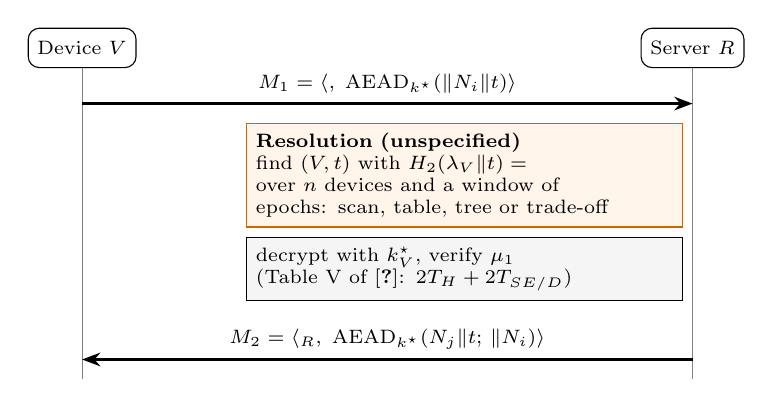
\begin{tikzpicture}[font=\scriptsize, >=Stealth, node distance=4mm]
\node[draw, rounded corners, minimum width=1.3cm, minimum height=5mm] (D) {Device $V$};
\node[draw, rounded corners, minimum width=1.3cm, minimum height=5mm, right=\flowgap of D] (S) {Server $R$};
\draw[gray] (D.south) -- ++(0,-3.95);
\draw[gray] (S.south) -- ++(0,-3.95);
\draw[->, thick] ($(D.south)+(0,-0.45)$) -- node[above, align=center]{$M_1=\langle \PID,\;\mathrm{AEAD}_{k^\star}(\PID\|N_i\|t)\rangle$} ($(S.south)+(0,-0.45)$);
\node[draw=orange!80!black, fill=orange!8, align=left, anchor=north east, text width=\flowtw] (R) at ($(S.south)+(-0.12,-0.7)$)
 {\textbf{Resolution (unspecified)}\\ find $(V,t)$ with $H_2(\lambda_V\|t)=\PID$\\ over $n$ devices and a window of\\ epochs: scan, table, tree or trade-off};
\node[draw, fill=gray!8, align=left, anchor=north east, text width=\flowtw] (V) at ($(R.south east)+(0,-0.12)$)
 {decrypt with $k^\star_V$, verify $\mu_1$\\ (Table~V of~\cite{base}: $2T_H+2T_{SE/D}$)};
\draw[<-, thick] ($(D.south)+(0,-3.7)$) -- node[above]{$M_2=\langle \ID_R,\;\mathrm{AEAD}_{k^\star}(N_j\|t;\,\PID\|N_i)\rangle$} ($(S.south)+(0,-3.7)$);
\end{tikzpicture}
\caption{Position of pseudonym resolution in the exchange. The server needs $k^\star_V$ to open $M_1$, but $V$ is hidden behind $\PID$.}
\label{fig:flow}
\end{figure}

\section{Design Space}\label{sec:design}
We implemented seven strategies (\designref), which we label O1 to O4, TM, CR and MW. The first five keep the wire
format of $M_1$. The last two need a fresh $r$ in clear, so they change $M_1$. They are modelled at the resolution level,
with the same keyed hash.
\begin{itemize}
\item \textbf{O1}, counter with a linear scan, is the behaviour of our original implementation. For each device it probes
epochs $\ell-L$ to $\ell+F$, where $\ell$ is the last accepted epoch, $L=16$ is the number of epochs below $\ell$ that the
server still checks (the replay lookback) and $F=8$ the number of epochs above it (the forward tolerance). The window is
$W=L+F+1=25$ epochs.
\item \textbf{O2} keeps a table of every device's next $F$ pseudonyms and slides it after each acceptance.
\item \textbf{O3} and \textbf{O4} use clock epochs with a drift window $\Wc=3$ (the current epoch and one on each side).
O3 scans, and O4 extends a table once per epoch.
\item \textbf{TM}, the time-memory trade-off, is a rainbow table over $S=nm$ points, with lifetime $m=128$ epochs per
device, chain length $S^{1/3}$ rounded to the nearest integer, $2S^{2/3}$ chains per table, and six tables.
\item \textbf{CR}, the challenge-response randomised hash lock, adds a fresh 128-bit $r$ to $M_1$ and tries every enrolled
key in turn. It keeps no resolution state and has no epochs.
\item \textbf{MW}, the key tree of Molnar and Wagner, uses branching factor $\delta=32$ and depth $d$, the number of tree
levels. For $n\le1{,}024$ the tree has $d\le2$ levels. The device adds $r$ and $d-1$ tags to $M_1$.
\end{itemize}

\ifspringer
\floatstart{table}
\centering
\caption{Design space, cost. $n$: devices enrolled at the server; $L=16$, $F=8$, $W=L+F+1$; $\Wc=3$; $S=nm$; $d$: depth of the
MW tree. ``Probes'' are expected $H_2$ evaluations per message, in steady state.}
\label{tab:design}
\footnotesize
\setlength{\tabcolsep}{2pt}
\begin{tabular}{@{}l l p{2.7cm} p{2.3cm} l@{}}
\toprule
Strategy & Epoch / $M_1$ & Probes, honest & Probes, forged & Precompute \\
\midrule
O1 & counter / unchanged & $\frac{(n-1)W}{2}+L+2$ & $nW$ & none \\
O2 & counter / unchanged & $1$ (slide) & $0$ & $nF$ once \\
O3 & clock / unchanged & $\frac{(n-1)\Wc}{2}+1$ & $n\Wc$ & none \\
O4 & clock / unchanged & $0$ & $0$ & $n$ per epoch \\
TM & counter / unchanged & $\approx0.5$--$0.7\,S^{2/3}$ (meas.) & $\approx4\,S^{2/3}$ (meas.) & $\approx12S$ once \\
CR & none / $+r$ (128 bits) & $\frac{n+1}{2}$ & $n$ & none \\
MW & none / $+r$, $+(d-1)$ tags & $\le\delta d$ & $\le\delta$ & none \\
\bottomrule
\end{tabular}
\end{table}

\floatstart{table}
\centering
\caption{Design space, state and behaviour (same strategies as Table~\ref{tab:design}). One table entry is 40 bytes and one
nonce-cache entry 24 bytes.}
\label{tab:designb}
\footnotesize
\setlength{\tabcolsep}{3pt}
\begin{tabular}{@{}l l l l@{}}
\toprule
Strategy & Resolution state & Dropped $M_1$ & Linkability \\
\midrule
O1 & $8n$ bytes & lockout after $F$ & none \\
O2 & $(40F+8)n$ bytes & lockout after $F$ & none \\
O3 & $24n$ bytes (nonce cache) & none & same epoch \\
O4 & $(40\Wc+24)n$ bytes & none & same epoch \\
TM & $\approx50\,S^{2/3}$ bytes & none until $t=m$ & none \\
CR & none & none & none \\
MW & 32 bytes per internal node & none & after compromise \\
\bottomrule
\end{tabular}
\end{table}
\else
\floatstart{table*}
\centering
\caption{Design space. $n$: devices enrolled at the server; $L=16$, $F=8$, $W=L+F+1$; $\Wc=3$; $S=nm$; $d$: depth of the
MW tree. One table entry is 40 bytes and one nonce-cache entry 24 bytes. ``Probes'' are expected $H_2$ evaluations per
message, in steady state.}
\label{tab:design}
\footnotesize
\setlength{\tabcolsep}{2.4pt}
\begin{tabular}{@{}l l l l l l l l@{}}
\toprule
Strategy & Epoch / $M_1$ & Probes, honest & Probes, forged & Precompute & Resolution state & Dropped $M_1$ & Linkability \\
\midrule
O1 & counter / unchanged & $\frac{(n-1)W}{2}+L+2$ & $nW$ & none & $8n$ bytes & lockout after $F$ & none \\
O2 & counter / unchanged & $1$ (slide) & $0$ & $nF$ once & $(40F+8)n$ bytes & lockout after $F$ & none \\
O3 & clock / unchanged & $\frac{(n-1)\Wc}{2}+1$ & $n\Wc$ & none & $24n$ bytes (nonce cache) & none & same epoch \\
O4 & clock / unchanged & $0$ & $0$ & $n$ per epoch & $(40\Wc+24)n$ bytes & none & same epoch \\
TM & counter / unchanged & $\approx0.5$--$0.7\,S^{2/3}$ (meas.) & $\approx4\,S^{2/3}$ (meas.) & $\approx12S$ once & $\approx50\,S^{2/3}$ bytes & none until $t=m$ & none \\
CR & none / $+r$ (128 bits) & $\frac{n+1}{2}$ & $n$ & none & none & none & none \\
MW & none / $+r$, $+(d-1)$ tags & $\le\delta d$ & $\le\delta$ & none & 32 bytes per internal node & none & after compromise \\
\bottomrule
\end{tabular}
\end{table*}
\fi

\section{Evaluation Method}\label{sec:method}
We follow the base paper's evaluation conditions and change only the resolution term.
\begin{itemize}
\item \emph{Simulator and environment}: OMNeT++ 6.4~\cite{omnet} (Cmdenv), with Table~II of~\cite{base}: a
1{,}500\,m $\times$ 1{,}500\,m area, 10\,Mb/s, 500\,m range, 75.6\,mW, a 15\,\textmu s quantum, servers at 5\% of the devices.
\item \emph{Protocol cost}: Tables~III--V of~\cite{base}. That is $2T_H+2T_{SE/D}=11.84$\,ms per side, $T_H=0.32$\,ms per
probe, and 1{,}024 bits, which Table~IV of~\cite{base} lists for four messages although the protocol has two.
\item \emph{Resolution cost}: for each server we look up the probes for its number of enrolled devices $n$ in the
measured cost model. It is exact for O1--O4 and CR, and interpolated between measured points for TM and MW. CR and MW
also add their extra $M_1$ bits. At $N\ge100$ each server enrols about a quarter of the devices ($n\approx258$ at
$N=1{,}000$).
\item \emph{Assumptions} (the base paper does not fix these): an adversary share of 5\%, each sending forged $M_1$ at
1\,Hz; a 10\,s window in which each device starts one authentication; \emph{reachable enrolment}, in which each server
enrols every device in its radio range (the alternative, \emph{nearest enrolment}, enrols each device only at the server
nearest to it); first-come-first-served server processing; for O4, one epoch extension per server inside the window.
\item \emph{Runs}: five seeds per point, at 12 network sizes ($N=1$, 10, 100, and 200 to 1{,}000 in steps of 100), and eight
configurations: the seven strategies and, as the eighth, the baseline without resolution. Each is run with and without
adversaries. That is $12\times8\times5\times2=960$ runs, reported as means.
\end{itemize}

The model is ours, not the authors' (\secref{sec:validation} gives its validation, and \secref{sec:sens} the effect of
these assumptions). The base column of \tabref{tab:ranked} ($N=1$) is therefore the base paper's own figure: 23.68\,ms from
Tables~III and~V of~\cite{base}, and 320 bits (40 bytes) of server storage from Table~VI of~\cite{base}. Latency in \tabref{tab:ranked}
is the mean per-session latency over five seeds. Storage at larger $N$ is those 320 bits per enrolled device plus the
resolution state, averaged over the servers of the simulated network; 1\,KiB is 1{,}024 bytes throughout.

\section{Validation}\label{sec:validation}
Each result rests on one of these checks, all of which can be rerun from the repository.
\begin{itemize}
\item \emph{Protocol implementation.} The Python implementation and the C port of the device side reproduce reference
vectors byte for byte (15 checks each). The vectors were computed by a generator that shares no code with either
implementation. They cover the pairwise key, the pseudonym, the wire bytes of $M_1$ and $M_2$, and the session key,
together with the rejection of tampered and replayed messages. A C device and the Python server complete five handshakes
with matching session keys, and the server rejects a replayed $M_1$. All 125 unit and property tests pass.
\item \emph{Resolution strategies.} For each strategy and each
$n\in\{$1, 2, 5, 10, 20, 50, 100, 200, 300, 500, 700, 1{,}000, 2{,}000, 5{,}000, 10{,}000$\}$ (15 values), a script builds the server in
steady state. It resolves 200 pseudonyms of randomly drawn devices (50 for O1, O3, TM and CR above $n=2{,}000$) and five
forged ones, and counts every $H_2$ call. For O1--O4 and CR, the forged and per-epoch counts and the state equal the closed
forms of \designref exactly. O2 and O4 need exactly 1 and 0 probes per authentication. The honest means of O1, O3
and CR lie within four standard errors of the formulas, and MW never exceeds $\delta d$. In our parameter runs ($n=40$ to
500), the TM tables covered 99.6--99.8\% of points. In the sweep, they missed 9 of 2{,}100 honest pseudonyms, the samples
at the 12 sizes with $n\ge10$ (10 sizes with 200 pseudonyms and 2 with 50); the device then retries with its next epoch.
A total of 12 unit tests run each wire-compatible strategy through the full handshake and check its probe counts, replay rejection and
lockout. A rerun of the sweep reproduced every non-TM count exactly; TM varies because its peer secrets are random.
\item \emph{Network model.} With the resolution term removed, the model gives 23.86\,ms at $N=1$ and 24.07\,ms at
$N=1{,}000$, against the base paper's arithmetic value of 23.68\,ms. The 0.8--1.7\% difference is airtime and
quantisation, which the arithmetic leaves out. In the baseline row of \tabref{tab:sens}, the load of the mean server,
computed independently of the simulator from the cost model, orders the strategies exactly as the simulation does
(\secref{sec:sens}).
\iffv
\ifshortpaper\else
\item \emph{Security properties.} ProVerif checks the security claims symbolically (\secref{sec:fv}).
\fi
\fi
\end{itemize}

\runin{Limits of the validation.} The code of the base paper is not available, so the vectors encode our reading of
Section~III of~\cite{base}: both implementations agree with that reading, which may not be what its authors intended. The
network model is checked against the base paper only at one device without resolution, the one point where it gives a
figure, and its saturated behaviour has not been compared with another simulator.

\section{Results}\label{sec:results}
\ifspringer
\floatstart{table}
\centering
\caption{Strategies ranked from best to worst by mean session latency at $N=1{,}000$ (5\% adversaries), in the OMNeT++
model of the network of Table~II of~\cite{base} with the constants of its Table~III (\secref{sec:method}). Storage: mean per
server. The base column ($N=1$) is the value published in~\cite{base}: 23.68\,ms and 320 bits.}
\label{tab:ranked}
\footnotesize
\setlength{\tabcolsep}{2pt}
\ifshortpaper
\begin{tabular}{@{}c l r r r r r@{\hspace{9pt}}r r r r r@{}}
\toprule
 & & \multicolumn{5}{c}{Mean session latency (ms), by $N$} & \multicolumn{5}{c}{Storage per server (KiB), by $N$} \\
\cmidrule(lr){3-7}\cmidrule(l){8-12}
\# & Strategy & base & 10 & 100 & 500 & 1{,}000 & base & 10 & 100 & 500 & 1{,}000 \\
\midrule
\rankedlsrows
\bottomrule
\end{tabular}
\else
\begin{tabular}{@{}c l l l@{}}
\toprule
\# & Strategy & Time per auth. & Space per auth. \\
\midrule
\rankedcomprows
\bottomrule
\end{tabular}

\medskip
\begin{tabular}{@{}c l r r r r r@{}}
\toprule
 & & \multicolumn{5}{c}{Mean session latency (ms), by $N$} \\
\cmidrule(l){3-7}
\# & Strategy & base & 10 & 100 & 500 & 1{,}000 \\
\midrule
\rankedlatrows
\bottomrule
\end{tabular}

\medskip
\begin{tabular}{@{}c l r r r r r@{}}
\toprule
 & & \multicolumn{5}{c}{Storage per server (KiB), by $N$} \\
\cmidrule(l){3-7}
\# & Strategy & base & 10 & 100 & 500 & 1{,}000 \\
\midrule
\rankedstorrows
\bottomrule
\end{tabular}
\fi
\end{table}
\else
\floatstart{table*}
\centering
\caption{Strategies ranked from best to worst by mean session latency at $N=1{,}000$ (5\% adversaries), in the OMNeT++
model of the network of Table~II of~\cite{base} with the constants of its Table~III (\secref{sec:method}). Storage: mean per
server. The base column ($N=1$) is the value published in~\cite{base}: 23.68\,ms and 320 bits.}
\label{tab:ranked}
\footnotesize
\setlength{\tabcolsep}{2pt}
\begin{tabular}{@{}c l l l l r r r r r r r r r r@{}}
\toprule
 & & & \multicolumn{2}{c}{Complexity per auth.} & \multicolumn{5}{c}{Mean session latency (ms), by $N$} & \multicolumn{5}{c}{Storage per server (KiB), by $N$} \\
\cmidrule(lr){4-5}\cmidrule(lr){6-10}\cmidrule(l){11-15}
\# & & Strategy & Time & Space & base & 10 & 100 & 500 & 1{,}000 & base & 10 & 100 & 500 & 1{,}000 \\
\midrule
\rankedrows
\bottomrule
\end{tabular}
\end{table*}
\fi

\floatstart{figure*}
\centering
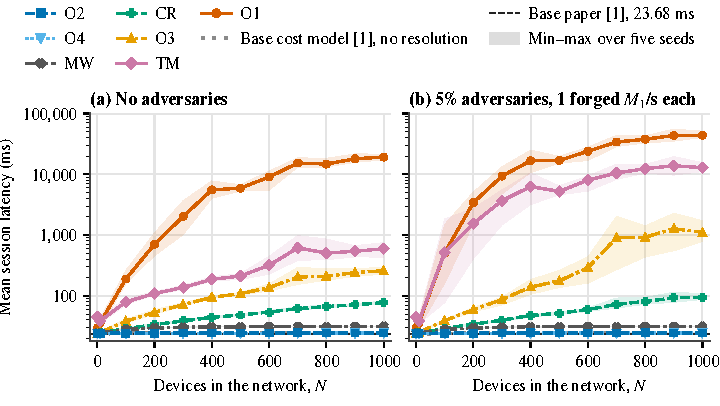
\includegraphics[width=\textwidth]{figs/fig_latency.pdf}
\caption{Mean session latency against network size in the OMNeT++ model (log scale; band: minimum to maximum over five
seeds). (a) Without adversaries. (b) With 5\% adversaries, each sending one forged $M_1$ per second. Dotted: the cost model of~\cite{base} with no resolution. Dashed: the base paper's 23.68\,ms.}
\label{fig:latency}
\end{figure*}

\subsection{Ranking}
\tabref{tab:ranked} gives the ranking. The two table strategies, O2 and O4, stay within 1\,ms of the base paper's figure up
to 1{,}000 devices. O2 needs one probe to slide the window, and O4 only the per-epoch extension. Their cost is memory: at
1{,}000 devices, about 93\,KiB and 46\,KiB per server, against 10\,KiB for Table~VI of~\cite{base} alone. The key tree is
third (31.4\,ms). It changes $M_1$, and a compromised device leaks the internal keys it shares with others. The
randomised hash lock (CR) needs no extra state, but its latency grows linearly, to 95\,ms. The three scanning strategies
with epochs saturate the server: clock scan (O3) at 1.1\,s, the time-memory trade-off at 12.9\,s, and the counter scan
(O1) at 44\,s. For O1 and TM, the spread across seeds at $N=1{,}000$ is 10.6\,s and 4.5\,s, because the latency depends on
how many devices and adversaries share the busiest server.

\subsection{Honest Load Against Forged Load}\label{sec:probes}
\figref{fig:latency} separates the two causes. Without adversaries (a), O1 already reaches 19.2\,s at 1{,}000 devices.
Each honest authentication costs about $12.5\,n$ probes, which is 1.0\,s of hashing at the $n\approx258$ devices that a
server enrols at $N=1{,}000$ ($T_H=0.32$\,ms). Arrivals outpace this, so the server queue grows. The forged load (b)
roughly doubles this, because every forged pseudonym costs a full miss scan of $Wn$ probes. Such a pseudonym never resolves
to a device, so the block-list, which blocks a device after three consecutive failed attempts, never sees it.
\figref{fig:probes} shows the same effect for one server enrolling up to $n=10{,}000$ devices. A forgery costs O1 250,000
probes and TM about 46,000, but costs O2 and O4 nothing, because a table miss needs no hash.

\floatstart{figure*}
\centering
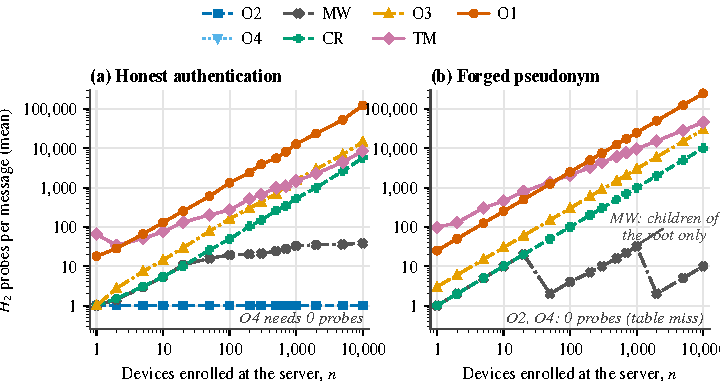
\includegraphics[width=\textwidth]{figs/fig_probes.pdf}
\caption{Probes per message at one server, measured on the implementation (log-log). (a) Honest authentication. (b) A
forged, random pseudonym.}
\label{fig:probes}
\end{figure*}

\subsection{Time Against Memory}
\figref{fig:storage} shows storage at one server, and each strategy's position in the time-memory plane for one server
enrolling $n=1{,}000$ devices. Storage is the resolution state plus the 40 bytes (320 bits) per device of Table~VI
of~\cite{base}. No strategy that keeps the wire format is both fast and small. O2 buys constant time with $F$ table entries
per device (359\,KiB in total), and O4 with $\Wc$ entries per device (180\,KiB). TM sits in between, at 167\,KiB and 1{,}478
probes. It is dominated here because its table must cover the device's whole lifetime ($m=128$ epochs), not just the
current window. MW is the only point that is both small and fast, and it pays with a different $M_1$ and a weaker privacy
model.

\floatstart{figure*}
\centering
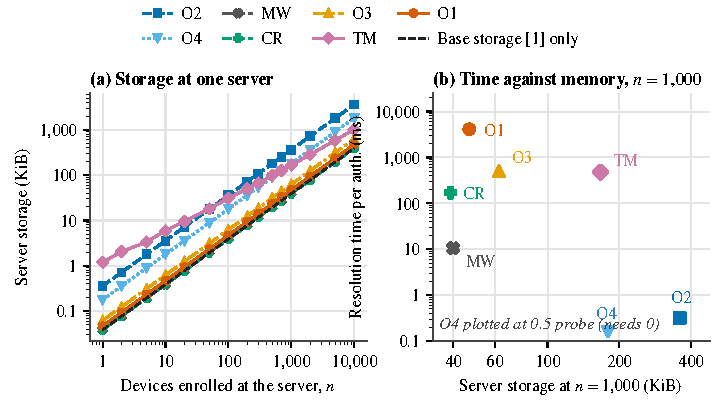
\includegraphics[width=\textwidth]{figs/fig_storage.pdf}
\caption{(a) Server storage (the 320 bits per device of Table~VI of~\cite{base} plus the resolution state) for one server.
(b) Resolution time per authentication ($T_H=0.32$\,ms per probe) against storage, for one server enrolling 1{,}000
devices.}
\label{fig:storage}
\end{figure*}

\subsection{Desynchronisation}\label{sec:desync}
With counter epochs, the device advances $t$ every time it builds $M_1$. The server searches at most $F$ epochs ahead of
the last one it accepted. In our implementation, an adversary who drops $F=8$ consecutive $M_1$ messages locks the device
out for good: every later handshake fails with an unknown pseudonym, with or without an earlier successful session. The
lockout holds for O1 and O2, and a unit test checks it for both. The threshold is $F$, which the specification does not
fix. A larger $F$ delays the lockout but does not remove it. A device whose counter lives in RAM is also rejected as
a replay after a restart; we observed this for O1. Message dropping is within the threat model of~\cite{base}. Clock epochs
(O3, O4), CR and MW have no per-device counter, so they cannot desynchronise this way. TM tolerates any number of drops
until $t$ reaches the lifetime $m$.

\subsection{Sensitivity to the Assumptions}\label{sec:sens}
The base paper does not fix the adversary share and rate, the authentication window or the enrolment rule, and $T_H$ is its
constant, not our measurement. We bound their effect without new simulation runs. First, the simulation was run with and
without adversaries (\figref{fig:latency}): at $N=1{,}000$ the ranking is the same, and O2, O4 and MW move by less than
0.2\,ms. Second, we compute the offered load of the mean server at $N=1{,}000$ from the committed cost model,
$\rho=\alpha_h(C_R+hT_H)+\alpha_a fT_H$, where $C_R=11.84$\,ms is the server cost per session from Tables~III and~V of~\cite{base},
$h$ and $f$ are the measured honest and forged probes at the mean enrolment $n=258$, and $\alpha_h$ and $\alpha_a$ are the
honest and forged arrival rates per server. $\rho\ge1$ means saturation (\tabref{tab:sens}).

\floatstart{table}
\centering
\caption{Offered load $\rho$ of the mean server at $N=1{,}000$, one assumption varied at a time from the baseline (5\%
adversaries at 1\,Hz, 10\,s window, reachable enrolment, $T_H=0.32$\,ms). $\rho\ge1$: saturated.}
\label{tab:sens}
\footnotesize
\setlength{\tabcolsep}{2.6pt}
\begin{tabular}{@{}l r r r r r r r@{}}
\toprule
Case & O2 & O4 & MW & CR & O3 & TM & O1 \\
\midrule
Baseline              & 0.02 & 0.03 & 0.04 & 0.19 & 0.52 & 1.68 & 4.16 \\
No adversaries        & 0.02 & 0.03 & 0.04 & 0.11 & 0.27 & 0.41 & 2.09 \\
20\% adversaries      & 0.02 & 0.03 & 0.05 & 0.44 & 1.26 & 5.47 & 10.3 \\
Adversary rate 2\,Hz  & 0.02 & 0.03 & 0.04 & 0.27 & 0.77 & 2.94 & 6.22 \\
Window 5\,s           & 0.05 & 0.06 & 0.08 & 0.30 & 0.79 & 2.09 & 6.25 \\
Window 20\,s          & 0.01 & 0.02 & 0.02 & 0.14 & 0.38 & 1.47 & 3.11 \\
$T_H=0.16$\,ms        & 0.02 & 0.03 & 0.03 & 0.11 & 0.27 & 0.85 & 2.09 \\
$T_H=0.64$\,ms        & 0.03 & 0.04 & 0.06 & 0.36 & 1.01 & 3.33 & 8.29 \\
Nearest enrolment     & 0.02 & 0.02 & 0.04 & 0.04 & 0.06 & 0.36 & 0.35 \\
\bottomrule
\end{tabular}
\end{table}

Except in the last row, the order by $\rho$ is that of \tabref{tab:ranked}, and O2 and O4 do not exceed 0.06. The
absolute figures do depend on the assumptions: O1 saturates unless $T_H<0.076$\,ms, and O3 saturates with 20\%
adversaries or $T_H=0.64$\,ms. (The busiest server enrols up to 396 devices, which is why O3 already queues in the
simulation at $\rho=0.52$.) If a server enrols only the devices attached to it ($n\approx20$), nothing saturates and the
lower ranks reorder, but O2 and O4 stay first. $L$, $F$ and $\Wc$ act only through the closed forms of
\designref. The recommendation of \secref{sec:disc} therefore holds under every assumption we varied, while
figures such as O1's 44\,s hold only under the baseline.

\iffv
\section{Formal Verification}\label{sec:fv}
We modelled the exchange in ProVerif~2.05~\cite{proverif}, in the symbolic model with an active attacker
(\tabref{tab:fv}). Other lightweight IoT schemes are checked in the same tool~\cite{wu22,lee25}; the scheme of~\cite{lee25},
for example, proves the privacy of its pseudonyms in ProVerif~2.05. Our hash, KDF and AEAD are free functions, and AEAD has
associated data. The main model has unbounded servers, unbounded honest and corrupt devices per server, and unbounded
sessions. A corrupt device's $\lambda$ and $k^\star$ are given to the attacker. The server may resolve a pseudonym to
\emph{any} enrolled device, and must then decrypt and check $\PID=H_2(\lambda_V\|t)$. So every result that holds, holds for
every resolver that returns a correct device. Epochs are fresh values, and the server keeps no replay state. Unlinkability
is checked as observational equivalence~\cite{blanchet08}, in the style of~\cite{arapinis}: one device running twice,
against two devices running once each. On both sides the server knows both devices and resolves with one destructor.

\floatstart{table}
\centering
\caption{ProVerif results (all models finish in under 1\,s).}
\label{tab:fv}
\footnotesize
\begin{tabular}{@{}l p{3.6cm} p{2.6cm}@{}}
\toprule
Query & Property & Result \\
\midrule
Q1, Q2 & Session key secret (device and server side) & holds \\
Q3 & Server accepts $M_1$ of honest $V$ $\Rightarrow$ $V$ sent it & holds \\
Q4 & Same, injective & fails (replay, no replay state) \\
Q5 & Device accepts $M_2$ $\Rightarrow$ server derived the same key, injective & holds \\
FS & Forward secrecy: key secret after later leak of $k^\star$ & fails (leak reveals the nonces) \\
U1 & Unlinkability, counter epochs & holds \\
U2 & Unlinkability, clock epochs, same epoch & fails (equal $\PID$s) \\
\bottomrule
\end{tabular}
\end{table}

These results separate the properties that the resolver cannot affect from those it decides:
\begin{itemize}
\item \emph{Independent of the resolver}: secrecy of the session key (Q1, Q2), agreement on $(V,R,N_i,t)$ (Q3), and
injective key agreement for the device (Q5). Q5 holds because $N_i$ is fresh and bound as associated data of $M_2$.
\item \emph{Decided by the epoch and replay choices}: injective authentication of the device (Q4) fails without replay
state. ProVerif finds a trace in which one $M_1$ is accepted twice. Injectivity therefore rests on the epoch window (O1,
O2, TM) or the nonce cache (O3, O4), which the specification leaves open. Tamarin analyses of EDHOC likewise find that not
all of its methods satisfy injective agreement~\cite{norrman21}. With clock epochs, the attacker links two sessions in one
epoch by testing their pseudonyms for equality (U2), a case of the tracking that TrackDev~\cite{budykho} formalises. With
counter epochs, the equivalence holds (U1).
\item \emph{Forward secrecy (FS)}: it does not hold, and the base paper does not claim it. A later leak of $k^\star$
reveals $N_i$, $N_j$ and $t$ from the ciphertexts, and with them the session key.
\end{itemize}

Q4 cannot be settled in ProVerif with the replay window included, because the window is mutable state. We check the
window by test instead, and leave a stateful proof (for example in Tamarin, as done for EDHOC~\cite{norrman23}) to future
work.
\fi

\section{Discussion}\label{sec:disc}
\runin{Deployment recommendation.} A server that uses counter epochs should precompute (O2). One probe per
authentication and no hashing on forged input remove both the scaling and the denial-of-service problem, at about
$40F$ bytes per device. The lockout after $F$ dropped messages remains, so the device needs a resynchronisation path, or
the server needs a larger $F$, which costs table space linearly. If devices have clocks, O4 is faster than O2 up to 500
devices in \tabref{tab:ranked} and needs half the memory of O2, although O2 is faster at 1{,}000 devices (24.40\,ms against
24.59\,ms). O4 makes sessions within one epoch linkable and needs a nonce cache for replay detection. The epoch length then
trades privacy against the per-epoch rebuild of $n$ probes. On-demand scanning (O1, O3) is acceptable only for small $n$
and a trusted network. With 5\% adversaries, O1 is already 21 times the base paper's per-session cost at 100 devices.

\ifshortpaper\else
\runin{Specification gaps.} The protocol needs three decisions that it does not state: the epoch
semantics, the resolution method, and the replay state that makes device authentication injective. Its cost model
needs a resolution term. That term is $(n-1)W/2+L+2$ probes for an on-demand counter scan, and at least one probe or
one table lookup for a precomputed table. Its storage model needs the table.
\fi

\section{Limitations}\label{sec:lim}
\begin{itemize}
\item The simulation is our model of the environment of the base paper; the model of its authors is not available. Our
adversary, window and enrolment assumptions set the saturated latencies of O1, O3 and TM but not the lead of O2 and O4;
beyond the adversary share, this is shown from the mean-server load, not new runs (\secref{sec:sens}).
\item We price probes with the constant of Table~III of~\cite{base} ($T_H=0.32$\,ms) and report no hardware timings.
\item CR and MW change $M_1$ and are modelled at the resolution level only. The TM parameters (six tables, $m=128$) are
one point of its trade-off curve.
\item Our epoch, window and table choices are ours, and conformance means agreement with our reading of Section~III
of~\cite{base}, which only its authors can confirm.
\iffv
\item The ProVerif results are symbolic and assume perfect primitives.
\else
\item We give no formal proof.
\fi
\end{itemize}

\section{Conclusion}\label{sec:concl}
We set out to determine how the unspecified resolution step of~\cite{base} can be filled and what the choice decides.
(i)~\emph{Requirement.} Every correct server must resolve the pseudonym before any cryptographic check. The specification
leaves open the epoch semantics, the resolution method and the replay state, and its cost model has no term for the step.
(ii)~\emph{Cost.} Under the base paper's own constants and network, the choice decides whether a session stays at its
23.68\,ms or reaches tens of seconds at 1{,}000 devices. Precomputed tables (O2, O4), the oldest answer from RFID private
identification, stay within 1\,ms of the published figure at 46--93\,KiB per server. The lead of O2 and O4 holds under every
assumption we varied, while the size of the slowdown depends on them.
(iii)~\emph{Failure modes.} With on-demand scanning, every forged pseudonym costs a full scan that the block-list never
sees, while a table rejects it with no hashing. Counter epochs lock a device out after $F$ dropped messages, so a
deployment needs a resynchronisation path.
\iffv
(iv)~\emph{Security.} Session-key secrecy and agreement do not depend on the resolver, while unlinkability and injective
device authentication depend on the epoch and replay choices.
\fi
\ifanonymous
The implementation, the counting scripts, the OMNeT++ model\iffv, the ProVerif models\fi{} and all results are open in
the repository (link withheld for anonymous review).
\else
The implementation, the counting scripts, the OMNeT++ model\iffv, the ProVerif models\fi{} and all results are open at
\url{https://github.com/jaykerkar0405/hybrid-ecc-iot-auth}.
\fi

\ifbibtexrefs
\ifanonymous\else
\begin{credits}
\subsubsection{\ackname} This work was carried out as part of the Capstone Project course during semesters 6 and 7 at
Vivekanand Education Society's Institute of Technology. No funding was received for this research.
\subsubsection{\discintname} The Capstone Project course requires students to protect their work by a patent, copyright or
trademark filing before publishing it. The authors have no other competing interests to declare.
\end{credits}
\fi
\bibliographystyle{splncs04}
\bibliography{../refs}
\else
\begin{thebibliography}{99}
\bibitem{base} A. Al-Rasheed, R. Khan, A. Ahmad, A. Saeed, F. Alturise, and S. Alkhalaf, ``A low-cost hybrid elliptic curve cryptography authentication protocol for trustworthy Internet of Things communication,'' \emph{IEEE Trans. Consum. Electron.}, vol.~72, no.~2, pp.~4483--4491, May 2026, \doi{10.1109/TCE.2026.3662053}
\bibitem{weis} S. A. Weis, S. E. Sarma, R. L. Rivest, and D. W. Engels, ``Security and privacy aspects of low-cost radio frequency identification systems,'' in \emph{Security in Pervasive Computing (SPC 2003)}, ser. Lecture Notes in Computer Science, vol.~2802. Springer, 2004, pp.~201--212, \doi{10.1007/978-3-540-39881-3_18}
\bibitem{ohkubo} M. Ohkubo, K. Suzuki, and S. Kinoshita, ``Cryptographic approach to `privacy-friendly' tags,'' in \emph{RFID Privacy Workshop}, MIT, Cambridge, MA, USA, Nov. 2003.
\bibitem{molnar} D. Molnar and D. Wagner, ``Privacy and security in library RFID: Issues, practices, and architectures,'' in \emph{Proc. 11th ACM Conf. Comput. Commun. Secur. (CCS)}, Oct. 2004, pp.~210--219, \doi{10.1145/1030083.1030112}
\bibitem{avoine05} G. Avoine and P. Oechslin, ``A scalable and provably secure hash-based RFID protocol,'' in \emph{Proc. 3rd IEEE Int. Conf. Pervasive Comput. Commun. Workshops (PerCom Workshops)}, 2005, pp.~110--114, \doi{10.1109/PERCOMW.2005.12}
\bibitem{ado05} G. Avoine, E. Dysli, and P. Oechslin, ``Reducing time complexity in RFID systems,'' in \emph{Selected Areas in Cryptography (SAC 2005)}, ser. Lecture Notes in Computer Science, vol.~3897. Springer, 2006, pp.~291--306, \doi{10.1007/11693383_20}
\bibitem{tsudik} G. Tsudik, ``YA-TRAP: Yet another trivial RFID authentication protocol,'' in \emph{Proc. 4th IEEE Int. Conf. Pervasive Comput. Commun. Workshops (PerCom Workshops)}, 2006, pp.~640--643, \doi{10.1109/PERCOMW.2006.152}
\bibitem{tiplea} F. L. \c{T}iplea and C. Hristea, ``Practically efficient RFID scheme with constant-time identification,'' in \emph{Proc. 18th Int. Conf. Secur. Cryptogr. (SECRYPT)}. SciTePress, 2021, pp.~495--506, \doi{10.5220/0010544804950506}
\bibitem{gcm} M. Dworkin, ``Recommendation for block cipher modes of operation: Galois/Counter Mode (GCM) and GMAC,'' NIST, NIST SP 800-38D, Nov. 2007, \doi{10.6028/NIST.SP.800-38D}
\bibitem{hkdf} H. Krawczyk and P. Eronen, ``HMAC-based extract-and-expand key derivation function (HKDF),'' IETF, RFC 5869, May 2010, \doi{10.17487/RFC5869}
\bibitem{fips180} National Institute of Standards and Technology, ``Secure hash standard (SHS),'' NIST, FIPS PUB 180-4, Aug. 2015, \doi{10.6028/NIST.FIPS.180-4}
\bibitem{hellman} M. E. Hellman, ``A cryptanalytic time-memory trade-off,'' \emph{IEEE Trans. Inf. Theory}, vol.~26, no.~4, pp.~401--406, Jul. 1980, \doi{10.1109/TIT.1980.1056220}
\bibitem{oechslin} P. Oechslin, ``Making a faster cryptanalytic time-memory trade-off,'' in \emph{Advances in Cryptology -- CRYPTO 2003}, ser. Lecture Notes in Computer Science, vol.~2729. Springer, 2003, pp.~617--630, \doi{10.1007/978-3-540-45146-4_36}
\bibitem{omnet} A. Varga and R. Hornig, ``An overview of the OMNeT++ simulation environment,'' in \emph{Proc. 1st Int. ICST Conf. Simul. Tools Techn. Commun. Netw. Syst. (SIMUTools)}. ICST, 2008, \doi{10.4108/ICST.SIMUTOOLS2008.3027}
\iffv
\bibitem{proverif} B. Blanchet, ``Modeling and verifying security protocols with the applied pi calculus and ProVerif,'' \emph{Found. Trends Privacy Secur.}, vol.~1, no.~1--2, pp.~1--135, Oct. 2016, \doi{10.1561/3300000004}
\bibitem{wu22} T.-Y. Wu, Q. Meng, S. Kumari, and P. Zhang, ``Rotating behind security: A lightweight authentication protocol based on IoT-enabled cloud computing environments,'' \emph{Sensors}, vol.~22, no.~10, Art. no.~3858, May 2022, \doi{10.3390/s22103858}
\bibitem{lee25} H. J. Lee, S. Kook, K. Kim, J. Ryu, Y. Lee, and D. Won, ``LAMT: Lightweight and anonymous authentication scheme for medical Internet of Things services,'' \emph{Sensors}, vol.~25, no.~3, Art. no.~821, Jan. 2025, \doi{10.3390/s25030821}
\bibitem{blanchet08} B. Blanchet, M. Abadi, and C. Fournet, ``Automated verification of selected equivalences for security protocols,'' \emph{J. Log. Algebr. Program.}, vol.~75, no.~1, pp.~3--51, Feb. 2008, \doi{10.1016/j.jlap.2007.06.002}
\bibitem{arapinis} M. Arapinis, T. Chothia, E. Ritter, and M. Ryan, ``Analysing unlinkability and anonymity using the applied pi calculus,'' in \emph{Proc. 23rd IEEE Comput. Secur. Found. Symp. (CSF)}, Jul. 2010, pp.~107--121, \doi{10.1109/CSF.2010.15}
\bibitem{norrman21} K. Norrman, V. Sundararajan, and A. Bruni, ``Formal analysis of EDHOC key establishment for constrained IoT devices,'' in \emph{Proc. 18th Int. Conf. Secur. Cryptogr. (SECRYPT)}. SciTePress, 2021, pp.~210--221, \doi{10.5220/0010554002100221}
\bibitem{budykho} K. Budykho \emph{et al.}, ``Fine-grained trackability in protocol executions,'' in \emph{Proc. Netw. Distrib. Syst. Secur. Symp. (NDSS)}. Internet Society, 2023, \doi{10.14722/ndss.2023.24289}
\bibitem{norrman23} K. Norrman, V. Sundararajan, and A. Bruni, ``Extended formal analysis of the EDHOC protocol in Tamarin,'' in \emph{E-Business and Telecommunications}, ser. Communications in Computer and Information Science. Springer, 2023, pp.~224--248, \doi{10.1007/978-3-031-36840-0_11}
\fi
\end{thebibliography}
\fi

\end{document}
".   \NOFV on the command line drops the formal-verification material.
\documentclass[runningheads]{llncs}
\newif\ifanonymous
\anonymoustrue   % <- the single switch: \anonymoustrue = review build, \anonymousfalse = camera-ready
\ifdefined\CAMERA\anonymousfalse\fi
\newif\iffv
\fvtrue
\ifdefined\NOFV\fvfalse\fi
\newif\ifshortpaper
\shortpapertrue
\newif\ifspringer
\springertrue
\newif\ifbibtexrefs
\bibtexrefstrue
\newcommand{\fpos}{!tb}
\renewcommand{\topfraction}{.85}\renewcommand{\bottomfraction}{.7}\renewcommand{\textfraction}{.1}\renewcommand{\floatpagefraction}{.7}                        % float placement: top or bottom of a page
\newcommand{\flowgap}{6.4cm}\newcommand{\flowtw}{5.3cm}   % Fig. 1 geometry (distance device-server, box text width)
\newcommand{\floatstart}[1]{\edef\floattmp{\noexpand\begin{#1}[\fpos]}\floattmp}   % \begin{#1}[placement]

\usepackage[T1]{fontenc}
\usepackage{amsmath,amssymb}
\usepackage{graphicx}
\usepackage{booktabs}
\usepackage{array}
\usepackage{textcomp}      % upright micro sign \textmu
\usepackage{url}
\usepackage{tikz}
\hfuzz=1pt                   % do not report sub-point overfull boxes
\setlength{\emergencystretch}{1em}   % only helps line breaking; no metric of the template changes
\usetikzlibrary{arrows.meta,positioning,calc}

% Cross-reference macros: "Sect. 7.5" (running text), "Section 7.5" (sentence start), "Fig. 2", "Table 2", "Eq. (1)".
% Pointers into the base paper are literal text in the body (e.g. "Table V of [1]") and do not use these.
\newcommand{\secref}[1]{Sect.~\ref{#1}}
\newcommand{\Secref}[1]{Section~\ref{#1}}
\newcommand{\secsref}[2]{Sects.~\ref{#1} and~\ref{#2}}
\newcommand{\figref}[1]{Fig.~\ref{#1}}
\newcommand{\tabref}[1]{Table~\ref{#1}}
\newcommand{\eqnref}[1]{Eq.~(\ref{#1})}
\newcommand{\designref}{Tables~\ref{tab:design} and~\ref{tab:designb}}
\newcommand{\runin}[1]{\paragraph{#1}}

% Keywords sit inside the abstract in llncs: 4-6 keywords, first letter capitalised.
\newcommand{\abstractkeywords}{%
\keywords{IoT authentication \and Pseudonym resolution \and Unlinkability \and Private identification \and Scalability%
\iffv \and ProVerif\fi}}
\newcommand{\afterabstract}{}

\begin{document}
\title{Pseudonym Resolution and Formal Verification of an Unlinkable Two-Message IoT Authentication Protocol}
\ifanonymous
  \titlerunning{Pseudonym Resolution in IoT Authentication}
  \author{Anonymous Author(s)}
  \authorrunning{Anonymous}
  \institute{Anonymous Institution}
  \pdfinfo{/Title (Pseudonym Resolution and Formal Verification of an Unlinkable Two-Message IoT Authentication Protocol) /Author ()}
\else
  \titlerunning{Pseudonym Resolution in IoT Authentication}
  \author{Jay Kerkar\inst{1}\orcidID{0009-0007-4612-6097} \and Chaitanya Kelkar\inst{1} \and Chirag Poornamath\inst{1} \and
  Yash Kolekar\inst{1} \and Shanta Sondur\inst{1}}
  \authorrunning{J. Kerkar et al.}
  \institute{Department of Information Technology, Vivekanand Education Society's Institute of Technology, Mumbai, India\\
  \email{jaykerkar0405@gmail.com, chaitanyakelkar07@gmail.com, chiragpoornamath@gmail.com, yashkolekar1234@gmail.com, shanta.sondur@ves.ac.in}}
  \pdfinfo{/Title (Pseudonym Resolution and Formal Verification of an Unlinkable Two-Message IoT Authentication Protocol) /Author (Jay Kerkar, Chaitanya Kelkar, Chirag Poornamath, Yash Kolekar, Shanta Sondur)}
\fi
\maketitle
% Copyright (c) 2026 Jay Kerkar, Chaitanya Kelkar, Chirag Poornamath, Yash Kolekar and Shanta Sondur
% SPDX-License-Identifier: Apache-2.0
% Shared body of all venue versions. \iffv ... \fi marks the material that only the version with formal verification contains.
% \ifanonymous (default false) removes everything that identifies the authors.
% Numbers come from figs/summary.json and figs/table_ranked.tex, written by make_figs.py.
%
% Contract with the wrapper (main.tex for IEEE, one wrapper per venue): before \input{body.tex} it defines
%   \iffv, \ifanonymous            switches
%   \ifspringer (single-column float layouts), \ifbibtexrefs (BibTeX list instead of the inline one), \runin, \Secref (sentence start), \designref, \abstractkeywords, \afterabstract (venue hooks)
%   \ifshortpaper (Springer page limit: drops the organisation paragraph, the complexity block of the ranked table and the "Specification gaps" paragraph)
%   \secref, \secsref, \figref, \tabref, \eqnref   venue-specific reference macros, e.g. \secref{x} -> "Section VII-E" (IEEE)
%                                  or "Sect. 7.5" (Springer). Pointers into the base paper are literal text and stay as they are.
% Springer camera-ready only (\ifbibtexrefs, not anonymous): the credits block before the references carries the funding,
% project-context and competing-interests statements supplied by the authors.
\newcommand{\PID}{\mathit{PID}}
\newcommand{\ID}{\mathit{ID}}
\newcommand{\Wc}{W_{\mathrm{c}}}
\def\rankedrows{%
1 & O2 & Counter + precomputed table  & $O(1)$ & $O(nF)$ & 23.68 & 24.17 & 24.25 & 24.40 & 24.40 & 0.04 & 0.93 & 8.78 & 46.1 & 92.9 \\
2 & O4 & Clock + per-epoch table \cite{tsudik} & $O(1)$, $+O(n)$ per epoch & $O(nW_{\mathrm{c}})$ & 23.68 & 23.85 & 23.93 & 24.22 & 24.59 & 0.04 & 0.47 & 4.39 & 23.1 & 46.4 \\
3 & MW & Key tree \cite{molnar} & $O(\delta\log_\delta n)$ & $O(n)$ & 23.68 & 24.44 & 27.96 & 30.86 & 31.38 & 0.04 & 0.10 & 0.97 & 5.16 & 10.4 \\
4 & CR & Randomised hash lock \cite{weis} & $O(n)$ & $O(n)$ & 23.68 & 24.44 & 28.86 & 51.71 & 94.89 & 0.04 & 0.10 & 0.95 & 5.02 & 10.1 \\
5 & O3 & Clock + linear scan  & $O(nW_{\mathrm{c}})$ & $O(n)$ & 23.68 & 24.94 & 38.99 & 176.1 & 1,108 & 0.04 & 0.16 & 1.53 & 8.03 & 16.1 \\
6 & TM & Rainbow time-memory trade-off \cite{avoine05,ado05} & $O((nm)^{2/3})$ & $O((nm)^{2/3})$ & 23.68 & 38.33 & 516.5 & 5,228 & 12,850 & 0.04 & 2.26 & 10.8 & 36.5 & 59.9 \\
7 & O1 & Counter + linear scan \cite{ohkubo} & $O(nW)$ & $O(n)$ & 23.68 & 36.02 & 507.9 & 16,947 & 44,010 & 0.04 & 0.12 & 1.15 & 6.02 & 12.1 \\
}
\def\rankedcomprows{%
1 & O2 Counter + precomputed table  & $O(1)$ & $O(nF)$ \\
2 & O4 Clock + per-epoch table \cite{tsudik} & $O(1)$, $+O(n)$ per epoch & $O(nW_{\mathrm{c}})$ \\
3 & MW Key tree \cite{molnar} & $O(\delta\log_\delta n)$ & $O(n)$ \\
4 & CR Randomised hash lock \cite{weis} & $O(n)$ & $O(n)$ \\
5 & O3 Clock + linear scan  & $O(nW_{\mathrm{c}})$ & $O(n)$ \\
6 & TM Rainbow time-memory trade-off \cite{avoine05,ado05} & $O((nm)^{2/3})$ & $O((nm)^{2/3})$ \\
7 & O1 Counter + linear scan \cite{ohkubo} & $O(nW)$ & $O(n)$ \\
}
\def\rankedlatrows{%
1 & O2 & 23.68 & 24.17 & 24.25 & 24.40 & 24.40 \\
2 & O4 & 23.68 & 23.85 & 23.93 & 24.22 & 24.59 \\
3 & MW & 23.68 & 24.44 & 27.96 & 30.86 & 31.38 \\
4 & CR & 23.68 & 24.44 & 28.86 & 51.71 & 94.89 \\
5 & O3 & 23.68 & 24.94 & 38.99 & 176.1 & 1,108 \\
6 & TM & 23.68 & 38.33 & 516.5 & 5,228 & 12,850 \\
7 & O1 & 23.68 & 36.02 & 507.9 & 16,947 & 44,010 \\
}
\def\rankedstorrows{%
1 & O2 & 0.04 & 0.93 & 8.78 & 46.1 & 92.9 \\
2 & O4 & 0.04 & 0.47 & 4.39 & 23.1 & 46.4 \\
3 & MW & 0.04 & 0.10 & 0.97 & 5.16 & 10.4 \\
4 & CR & 0.04 & 0.10 & 0.95 & 5.02 & 10.1 \\
5 & O3 & 0.04 & 0.16 & 1.53 & 8.03 & 16.1 \\
6 & TM & 0.04 & 2.26 & 10.8 & 36.5 & 59.9 \\
7 & O1 & 0.04 & 0.12 & 1.15 & 6.02 & 12.1 \\
}
\def\rankedlsrows{%
1 & O2 & 23.68 & 24.17 & 24.25 & 24.40 & 24.40 & 0.04 & 0.93 & 8.78 & 46.1 & 92.9 \\
2 & O4 & 23.68 & 23.85 & 23.93 & 24.22 & 24.59 & 0.04 & 0.47 & 4.39 & 23.1 & 46.4 \\
3 & MW & 23.68 & 24.44 & 27.96 & 30.86 & 31.38 & 0.04 & 0.10 & 0.97 & 5.16 & 10.4 \\
4 & CR & 23.68 & 24.44 & 28.86 & 51.71 & 94.89 & 0.04 & 0.10 & 0.95 & 5.02 & 10.1 \\
5 & O3 & 23.68 & 24.94 & 38.99 & 176.1 & 1,108 & 0.04 & 0.16 & 1.53 & 8.03 & 16.1 \\
6 & TM & 23.68 & 38.33 & 516.5 & 5,228 & 12,850 & 0.04 & 2.26 & 10.8 & 36.5 & 59.9 \\
7 & O1 & 23.68 & 36.02 & 507.9 & 16,947 & 44,010 & 0.04 & 0.12 & 1.15 & 6.02 & 12.1 \\
}


\begin{abstract}
Many lightweight IoT authentication protocols send an unlinkable pseudonym in clear and encrypt the rest under a
device-specific key, so the server must identify the sender before decrypting. We study this
resolution step for the two-message protocol of Al-Rasheed et al.\ (IEEE Transactions on Consumer Electronics, 2026), the
base paper. We show that every correct server needs the step, and that the base paper neither specifies nor costs it. We
implement the protocol, check it against independent reference vectors, and add seven resolution strategies: five that
keep the wire format, two that change the first message. Five adapt RFID privacy research. We measure probe counts and
price them with the base paper's constants in an OMNeT++ model of its network. Without resolution, our model
gives 23.86\,ms at one device, 0.8\% above the base paper's 23.68\,ms. At 1{,}000 devices with 5\%
adversaries, a precomputed table keeps the session at 24.4\,ms, while the on-demand scan reaches 44\,s, because each
forged pseudonym forces a full scan that no failure count sees. With counter epochs, a device that misses $F$
consecutive messages ($F=8$) is locked out for good. Varying our assumptions changes the absolute figures but not the
lead of the precomputed tables.
\iffv
ProVerif shows that session-key secrecy and agreement hold for every correct resolver, unlinkability holds with counter
epochs but fails with clock epochs, and injective device authentication needs replay state the specification leaves
open.
\fi
\ifanonymous
Code, models and data are open in the repository (link withheld for anonymous review).
\else
Code, models and data are open.
\fi
\abstractkeywords
\end{abstract}
\afterabstract


\section{Introduction}
Lightweight mutual-authentication protocols for IoT devices often hide the device's identity behind a pseudonym that
changes over time, so that an eavesdropper cannot link two sessions of the same device. Al-Rasheed et al.\ propose such a
protocol (IEEE Transactions on Consumer Electronics, 2026), which we call \emph{the base paper}~\cite{base}. Devices and
servers share pairwise keys from an offline phase, and they authenticate in two messages using symmetric primitives only;
the elliptic-curve operations from which the protocol takes its name belong to the offline phase. The device sends a
pseudonym $\PID=H_2(\lambda_V\|t)$, a hash of its long-term secret $\lambda_V$ and the epoch $t$, in clear. The epoch $t$
and the nonce $N_i$ travel inside a ciphertext under the pairwise key $k^\star$.

This design has a cost on the server side. The server cannot decrypt the first message until it knows which device sent
it, and the pseudonym is designed to hide exactly that. RFID privacy research has studied this tension for 20
years~\cite{weis,ohkubo,molnar,avoine05,ado05,tsudik}. It is known as \emph{private identification}: without
precomputation, a reader that must identify one of $n$ tags from an unlinkable response does $O(n)$ work. Recent RFID
work still aims at constant-time identification~\cite{tiplea}. In the base paper, the step is not specified, and its cost
model (Table~V and Eq.~22 of~\cite{base}) has no term for it. Its evaluation assigns the server a constant
$2T_H+2T_{SE/D}$ per session, whatever the number of devices; here $T_H=0.32$\,ms is the time of one hash and
$T_{SE/D}=5.6$\,ms the time of one symmetric encryption or decryption (Table~III of~\cite{base}).

\runin{Motivation.} Lightweight protocols are compared through the cost figures in their own evaluation tables. If a
step whose cost grows with the network is missing from those tables, the comparison favours the protocol for reasons that
do not survive deployment. We met this step while implementing the protocol: our first server had to scan every enrolled
device over a window of epochs for every incoming message, and that cost appears nowhere in~\cite{base}. An operator who
fills the step in the obvious way may therefore see sessions grow from milliseconds to seconds, or devices locked out,
with no warning from the published cost model.

\runin{Objective.} For the protocol of~\cite{base}, we set out to determine (i)~whether pseudonym resolution is required
and what the specification leaves open; (ii)~how the step can be filled, and what each choice costs in time and memory
as the network grows; (iii)~how each choice behaves under forged and dropped messages\iffv; and (iv)~which security
properties depend on the choice\fi. We answer these under the base paper's own constants and network, so that every result
can be compared directly with its published figures.

This paper makes the following contributions, which answer objective (i) (contribution~1), (ii) (2 and 3)\iffv, (iii)
(4) and (iv) (5)\else{} and (iii) (4)\fi:
\begin{enumerate}
\item \emph{The resolution gap.} From the specification alone, we show that every correct server must resolve the
pseudonym before any cryptographic check, and we state which choices the specification leaves open
(\secref{sec:gap}).
\item \emph{A design space.} We map seven strategies along the two open choices, the epoch semantics and the resolution
method: five that keep the wire format, and two that change the first message. Five of the seven adapt RFID work, and the
other two are ours. Each has a closed-form or measured cost (\secref{sec:design}).
\item \emph{A ranked comparison under the base paper's own conditions.} Probe counts measured on an open implementation
are priced with the constants of Table~III of~\cite{base}. They are evaluated in an OMNeT++ model of the network of
Table~II of~\cite{base}, and the one-device column is taken from the base paper itself. We also test how far the ranking
depends on our assumptions (\secref{sec:results}).
\item \emph{Failure modes.} We show the denial-of-service and desynchronisation behaviour of each strategy, including a
permanent lockout after $F$ dropped messages, which the threat model of the base paper allows
(\secsref{sec:probes}{sec:desync}).
\iffv
\item \emph{A formal analysis.} ProVerif models establish which security properties are independent of the resolver,
and which depend on the epoch and replay choices (\secref{sec:fv}).
\fi
\end{enumerate}

We do not re-evaluate the other results of~\cite{base}. We take its protocol as the specification and build on the parts
that we reproduced exactly.

\ifshortpaper\else
The rest of the paper is organised as follows. \Secref{sec:background} describes the protocol and the RFID work that we
adapt. \Secref{sec:gap} shows that resolution is required, and \secref{sec:design} defines the seven strategies.
\Secref{sec:method} describes the evaluation method, \secref{sec:validation} states how each result was validated, and
\secref{sec:results} gives the results.
\iffv
\Secref{sec:fv} presents the formal analysis.
\fi
\Secref{sec:disc} discusses the findings, \secref{sec:lim} lists the limitations, and \secref{sec:concl} concludes.
\fi

\section{Background}\label{sec:background}
\subsection{The Protocol}
In the offline phase, a trusted authority derives each entity's long-term secret $\lambda_X=H_1(\ID_X\|s)$ from the
entity's identifier $\ID_X$ and its master secret $s$. It gives each device--server pair the pairwise key
$k^\star=\mathrm{KDF}(\lambda_V\|\lambda_R)$, where KDF is a key derivation function (Eqs.~8--9 of~\cite{base}). Online,
in epoch $t$, the device $V$ samples $N_i$ and sends
\begin{equation*}
M_1=\langle\PID,\;\mathrm{AEAD}_{k^\star}(\PID\|N_i\|t)\rangle,\quad \PID=H_2(\lambda_V\|t).
\end{equation*}
AEAD is authenticated encryption with associated data; its authentication tag is the message authentication code
(MAC) $\mu_1$ of~\cite{base}. The server resolves $\PID$ to a device and an epoch, decrypts and verifies $M_1$, samples
$N_j$, and returns $M_2=\langle \ID_R,\mathrm{AEAD}_{k^\star}(N_j\|t;\,\PID\|N_i)\rangle$, where $\ID_R$ identifies the
server. Both sides derive $K=\mathrm{KDF}(k^\star\|N_i\|N_j\|t)$ (Eqs.~11--20 of~\cite{base}). We instantiate AEAD as
AES-256-GCM~\cite{gcm}, KDF as HKDF-SHA256 (HMAC-based KDF)~\cite{hkdf}, and both $H_1$ and $H_2$ as
SHA-256~\cite{fips180}, as the instantiation notes of~\cite{base} suggest. Our implementation adds no domain-separation
tag: $H_1$ hashes the identifier and the master secret, and $H_2$ hashes the 32-byte $\lambda$ and the epoch as an 8-byte
big-endian integer.

We implemented this exchange in Python, with a C port of the device side, and validated both against independent
reference vectors (\secref{sec:validation}). The vectors fix the message layout that the next section relies on: the
pseudonym is the only field in clear, and $N_i$ and $t$ are inside the AEAD ciphertext under $k^\star$.

\subsection{Private Identification in RFID}
The same problem appears when an RFID reader must identify a tag that answers with an unlinkable value. Five lines of work
define the strategies we adapt:
\begin{itemize}
\item \emph{Randomised hash lock}~\cite{weis}: the tag answers $(r, H(k\|r))$ for a fresh $r$, and the reader tries every
key, $O(n)$.
\item \emph{Hash chains} (OSK, after Ohkubo, Suzuki and Kinoshita)~\cite{ohkubo}: the tag's state evolves by a one-way
function, which gives forward privacy. The reader searches $n$ chains up to depth $m$, $O(nm)$. Our counter epochs are the
same search with the chain replaced by $H_2(\lambda\|t)$.
\item \emph{Key trees}~\cite{molnar}: keys form a tree of branching factor $\delta$, and the tag answers with one keyed
hash per level, $O(\delta\log_\delta n)$. Tags share their internal keys, so compromising one tag weakens the privacy of
others~\cite{ado05}.
\item \emph{Time-memory trade-off}~\cite{avoine05,ado05}: Hellman-style~\cite{hellman} rainbow tables~\cite{oechslin}
over all $(\text{tag},\ \text{state})$ pairs bring OSK to $O((nm)^{2/3})$ time and memory.
\item \emph{Time-based pseudonyms}, as in YA-TRAP~\cite{tsudik}: the reader precomputes one table per time period.
\end{itemize}

\ifshortpaper\else
Avoine et al.~\cite{ado05} compared these approaches by time and memory for one tag. \Secref{sec:results} makes the same
comparison for this protocol, at network scale and under the base paper's own constants.
\fi

\section{The Resolution Gap}\label{sec:gap}
\ifshortpaper\else
Each step of the argument uses only the specification, or a fact that our reference vectors confirm.
\fi
\begin{enumerate}
\item $M_1$ carries $\PID$ in clear. The epoch $t$ and nonce $N_i$ are only inside the ciphertext under $k^\star$
(Eqs.~13--15 of~\cite{base}; confirmed byte for byte).
\item $k^\star=\mathrm{KDF}(\lambda_V\|\lambda_R)$ is specific to the device (Eqs.~9 and 12 of~\cite{base}).
\item So the server cannot decrypt $M_1$ or verify its tag $\mu_1$ until it knows which device sent it.
\item The base paper requires that $\PID$ cannot be linked to $V$ without $\lambda_V$ (Section~III-J of~\cite{base}). So
the device's identity cannot be read from $M_1$ either.
\item So every correct server must map $\PID$ to $(V,t)$ by computing pseudonyms from the secrets it holds. We call this
step \emph{pseudonym resolution} (\figref{fig:flow}).
\end{enumerate}

The specification says only that the pseudonym is ``rotated with time (or epoch) $t$''. It leaves two choices open, and
together they decide the cost:
\begin{itemize}
\item \emph{Epoch semantics}: a per-device counter, or a clock.
\item \emph{Resolution method}: an on-demand search, or a table prepared in advance.
\end{itemize}

Table~V of~\cite{base} charges the server $2T_H+2T_{SE/D}$ per session, and Eq.~22 of~\cite{base} lists a fixed number of
KDF, encryption, decryption and MAC operations. Neither contains a term that grows with the number of devices. We count
resolution cost in \emph{probes}, where one probe is one evaluation of $H_2$ (or the equivalent keyed hash), and price it
at $T_H$ from Table~III of~\cite{base}. Throughout, $n$ is the number of devices enrolled at one server and $N$ the number
of devices in the network.

\floatstart{figure}
\centering
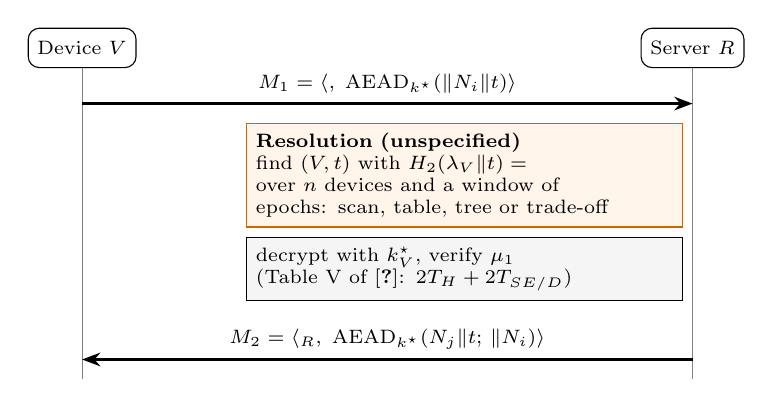
\begin{tikzpicture}[font=\scriptsize, >=Stealth, node distance=4mm]
\node[draw, rounded corners, minimum width=1.3cm, minimum height=5mm] (D) {Device $V$};
\node[draw, rounded corners, minimum width=1.3cm, minimum height=5mm, right=\flowgap of D] (S) {Server $R$};
\draw[gray] (D.south) -- ++(0,-3.95);
\draw[gray] (S.south) -- ++(0,-3.95);
\draw[->, thick] ($(D.south)+(0,-0.45)$) -- node[above, align=center]{$M_1=\langle \PID,\;\mathrm{AEAD}_{k^\star}(\PID\|N_i\|t)\rangle$} ($(S.south)+(0,-0.45)$);
\node[draw=orange!80!black, fill=orange!8, align=left, anchor=north east, text width=\flowtw] (R) at ($(S.south)+(-0.12,-0.7)$)
 {\textbf{Resolution (unspecified)}\\ find $(V,t)$ with $H_2(\lambda_V\|t)=\PID$\\ over $n$ devices and a window of\\ epochs: scan, table, tree or trade-off};
\node[draw, fill=gray!8, align=left, anchor=north east, text width=\flowtw] (V) at ($(R.south east)+(0,-0.12)$)
 {decrypt with $k^\star_V$, verify $\mu_1$\\ (Table~V of~\cite{base}: $2T_H+2T_{SE/D}$)};
\draw[<-, thick] ($(D.south)+(0,-3.7)$) -- node[above]{$M_2=\langle \ID_R,\;\mathrm{AEAD}_{k^\star}(N_j\|t;\,\PID\|N_i)\rangle$} ($(S.south)+(0,-3.7)$);
\end{tikzpicture}
\caption{Position of pseudonym resolution in the exchange. The server needs $k^\star_V$ to open $M_1$, but $V$ is hidden behind $\PID$.}
\label{fig:flow}
\end{figure}

\section{Design Space}\label{sec:design}
We implemented seven strategies (\designref), which we label O1 to O4, TM, CR and MW. The first five keep the wire
format of $M_1$. The last two need a fresh $r$ in clear, so they change $M_1$. They are modelled at the resolution level,
with the same keyed hash.
\begin{itemize}
\item \textbf{O1}, counter with a linear scan, is the behaviour of our original implementation. For each device it probes
epochs $\ell-L$ to $\ell+F$, where $\ell$ is the last accepted epoch, $L=16$ is the number of epochs below $\ell$ that the
server still checks (the replay lookback) and $F=8$ the number of epochs above it (the forward tolerance). The window is
$W=L+F+1=25$ epochs.
\item \textbf{O2} keeps a table of every device's next $F$ pseudonyms and slides it after each acceptance.
\item \textbf{O3} and \textbf{O4} use clock epochs with a drift window $\Wc=3$ (the current epoch and one on each side).
O3 scans, and O4 extends a table once per epoch.
\item \textbf{TM}, the time-memory trade-off, is a rainbow table over $S=nm$ points, with lifetime $m=128$ epochs per
device, chain length $S^{1/3}$ rounded to the nearest integer, $2S^{2/3}$ chains per table, and six tables.
\item \textbf{CR}, the challenge-response randomised hash lock, adds a fresh 128-bit $r$ to $M_1$ and tries every enrolled
key in turn. It keeps no resolution state and has no epochs.
\item \textbf{MW}, the key tree of Molnar and Wagner, uses branching factor $\delta=32$ and depth $d$, the number of tree
levels. For $n\le1{,}024$ the tree has $d\le2$ levels. The device adds $r$ and $d-1$ tags to $M_1$.
\end{itemize}

\ifspringer
\floatstart{table}
\centering
\caption{Design space, cost. $n$: devices enrolled at the server; $L=16$, $F=8$, $W=L+F+1$; $\Wc=3$; $S=nm$; $d$: depth of the
MW tree. ``Probes'' are expected $H_2$ evaluations per message, in steady state.}
\label{tab:design}
\footnotesize
\setlength{\tabcolsep}{2pt}
\begin{tabular}{@{}l l p{2.7cm} p{2.3cm} l@{}}
\toprule
Strategy & Epoch / $M_1$ & Probes, honest & Probes, forged & Precompute \\
\midrule
O1 & counter / unchanged & $\frac{(n-1)W}{2}+L+2$ & $nW$ & none \\
O2 & counter / unchanged & $1$ (slide) & $0$ & $nF$ once \\
O3 & clock / unchanged & $\frac{(n-1)\Wc}{2}+1$ & $n\Wc$ & none \\
O4 & clock / unchanged & $0$ & $0$ & $n$ per epoch \\
TM & counter / unchanged & $\approx0.5$--$0.7\,S^{2/3}$ (meas.) & $\approx4\,S^{2/3}$ (meas.) & $\approx12S$ once \\
CR & none / $+r$ (128 bits) & $\frac{n+1}{2}$ & $n$ & none \\
MW & none / $+r$, $+(d-1)$ tags & $\le\delta d$ & $\le\delta$ & none \\
\bottomrule
\end{tabular}
\end{table}

\floatstart{table}
\centering
\caption{Design space, state and behaviour (same strategies as Table~\ref{tab:design}). One table entry is 40 bytes and one
nonce-cache entry 24 bytes.}
\label{tab:designb}
\footnotesize
\setlength{\tabcolsep}{3pt}
\begin{tabular}{@{}l l l l@{}}
\toprule
Strategy & Resolution state & Dropped $M_1$ & Linkability \\
\midrule
O1 & $8n$ bytes & lockout after $F$ & none \\
O2 & $(40F+8)n$ bytes & lockout after $F$ & none \\
O3 & $24n$ bytes (nonce cache) & none & same epoch \\
O4 & $(40\Wc+24)n$ bytes & none & same epoch \\
TM & $\approx50\,S^{2/3}$ bytes & none until $t=m$ & none \\
CR & none & none & none \\
MW & 32 bytes per internal node & none & after compromise \\
\bottomrule
\end{tabular}
\end{table}
\else
\floatstart{table*}
\centering
\caption{Design space. $n$: devices enrolled at the server; $L=16$, $F=8$, $W=L+F+1$; $\Wc=3$; $S=nm$; $d$: depth of the
MW tree. One table entry is 40 bytes and one nonce-cache entry 24 bytes. ``Probes'' are expected $H_2$ evaluations per
message, in steady state.}
\label{tab:design}
\footnotesize
\setlength{\tabcolsep}{2.4pt}
\begin{tabular}{@{}l l l l l l l l@{}}
\toprule
Strategy & Epoch / $M_1$ & Probes, honest & Probes, forged & Precompute & Resolution state & Dropped $M_1$ & Linkability \\
\midrule
O1 & counter / unchanged & $\frac{(n-1)W}{2}+L+2$ & $nW$ & none & $8n$ bytes & lockout after $F$ & none \\
O2 & counter / unchanged & $1$ (slide) & $0$ & $nF$ once & $(40F+8)n$ bytes & lockout after $F$ & none \\
O3 & clock / unchanged & $\frac{(n-1)\Wc}{2}+1$ & $n\Wc$ & none & $24n$ bytes (nonce cache) & none & same epoch \\
O4 & clock / unchanged & $0$ & $0$ & $n$ per epoch & $(40\Wc+24)n$ bytes & none & same epoch \\
TM & counter / unchanged & $\approx0.5$--$0.7\,S^{2/3}$ (meas.) & $\approx4\,S^{2/3}$ (meas.) & $\approx12S$ once & $\approx50\,S^{2/3}$ bytes & none until $t=m$ & none \\
CR & none / $+r$ (128 bits) & $\frac{n+1}{2}$ & $n$ & none & none & none & none \\
MW & none / $+r$, $+(d-1)$ tags & $\le\delta d$ & $\le\delta$ & none & 32 bytes per internal node & none & after compromise \\
\bottomrule
\end{tabular}
\end{table*}
\fi

\section{Evaluation Method}\label{sec:method}
We follow the base paper's evaluation conditions and change only the resolution term.
\begin{itemize}
\item \emph{Simulator and environment}: OMNeT++ 6.4~\cite{omnet} (Cmdenv), with Table~II of~\cite{base}: a
1{,}500\,m $\times$ 1{,}500\,m area, 10\,Mb/s, 500\,m range, 75.6\,mW, a 15\,\textmu s quantum, servers at 5\% of the devices.
\item \emph{Protocol cost}: Tables~III--V of~\cite{base}. That is $2T_H+2T_{SE/D}=11.84$\,ms per side, $T_H=0.32$\,ms per
probe, and 1{,}024 bits, which Table~IV of~\cite{base} lists for four messages although the protocol has two.
\item \emph{Resolution cost}: for each server we look up the probes for its number of enrolled devices $n$ in the
measured cost model. It is exact for O1--O4 and CR, and interpolated between measured points for TM and MW. CR and MW
also add their extra $M_1$ bits. At $N\ge100$ each server enrols about a quarter of the devices ($n\approx258$ at
$N=1{,}000$).
\item \emph{Assumptions} (the base paper does not fix these): an adversary share of 5\%, each sending forged $M_1$ at
1\,Hz; a 10\,s window in which each device starts one authentication; \emph{reachable enrolment}, in which each server
enrols every device in its radio range (the alternative, \emph{nearest enrolment}, enrols each device only at the server
nearest to it); first-come-first-served server processing; for O4, one epoch extension per server inside the window.
\item \emph{Runs}: five seeds per point, at 12 network sizes ($N=1$, 10, 100, and 200 to 1{,}000 in steps of 100), and eight
configurations: the seven strategies and, as the eighth, the baseline without resolution. Each is run with and without
adversaries. That is $12\times8\times5\times2=960$ runs, reported as means.
\end{itemize}

The model is ours, not the authors' (\secref{sec:validation} gives its validation, and \secref{sec:sens} the effect of
these assumptions). The base column of \tabref{tab:ranked} ($N=1$) is therefore the base paper's own figure: 23.68\,ms from
Tables~III and~V of~\cite{base}, and 320 bits (40 bytes) of server storage from Table~VI of~\cite{base}. Latency in \tabref{tab:ranked}
is the mean per-session latency over five seeds. Storage at larger $N$ is those 320 bits per enrolled device plus the
resolution state, averaged over the servers of the simulated network; 1\,KiB is 1{,}024 bytes throughout.

\section{Validation}\label{sec:validation}
Each result rests on one of these checks, all of which can be rerun from the repository.
\begin{itemize}
\item \emph{Protocol implementation.} The Python implementation and the C port of the device side reproduce reference
vectors byte for byte (15 checks each). The vectors were computed by a generator that shares no code with either
implementation. They cover the pairwise key, the pseudonym, the wire bytes of $M_1$ and $M_2$, and the session key,
together with the rejection of tampered and replayed messages. A C device and the Python server complete five handshakes
with matching session keys, and the server rejects a replayed $M_1$. All 125 unit and property tests pass.
\item \emph{Resolution strategies.} For each strategy and each
$n\in\{$1, 2, 5, 10, 20, 50, 100, 200, 300, 500, 700, 1{,}000, 2{,}000, 5{,}000, 10{,}000$\}$ (15 values), a script builds the server in
steady state. It resolves 200 pseudonyms of randomly drawn devices (50 for O1, O3, TM and CR above $n=2{,}000$) and five
forged ones, and counts every $H_2$ call. For O1--O4 and CR, the forged and per-epoch counts and the state equal the closed
forms of \designref exactly. O2 and O4 need exactly 1 and 0 probes per authentication. The honest means of O1, O3
and CR lie within four standard errors of the formulas, and MW never exceeds $\delta d$. In our parameter runs ($n=40$ to
500), the TM tables covered 99.6--99.8\% of points. In the sweep, they missed 9 of 2{,}100 honest pseudonyms, the samples
at the 12 sizes with $n\ge10$ (10 sizes with 200 pseudonyms and 2 with 50); the device then retries with its next epoch.
A total of 12 unit tests run each wire-compatible strategy through the full handshake and check its probe counts, replay rejection and
lockout. A rerun of the sweep reproduced every non-TM count exactly; TM varies because its peer secrets are random.
\item \emph{Network model.} With the resolution term removed, the model gives 23.86\,ms at $N=1$ and 24.07\,ms at
$N=1{,}000$, against the base paper's arithmetic value of 23.68\,ms. The 0.8--1.7\% difference is airtime and
quantisation, which the arithmetic leaves out. In the baseline row of \tabref{tab:sens}, the load of the mean server,
computed independently of the simulator from the cost model, orders the strategies exactly as the simulation does
(\secref{sec:sens}).
\iffv
\ifshortpaper\else
\item \emph{Security properties.} ProVerif checks the security claims symbolically (\secref{sec:fv}).
\fi
\fi
\end{itemize}

\runin{Limits of the validation.} The code of the base paper is not available, so the vectors encode our reading of
Section~III of~\cite{base}: both implementations agree with that reading, which may not be what its authors intended. The
network model is checked against the base paper only at one device without resolution, the one point where it gives a
figure, and its saturated behaviour has not been compared with another simulator.

\section{Results}\label{sec:results}
\ifspringer
\floatstart{table}
\centering
\caption{Strategies ranked from best to worst by mean session latency at $N=1{,}000$ (5\% adversaries), in the OMNeT++
model of the network of Table~II of~\cite{base} with the constants of its Table~III (\secref{sec:method}). Storage: mean per
server. The base column ($N=1$) is the value published in~\cite{base}: 23.68\,ms and 320 bits.}
\label{tab:ranked}
\footnotesize
\setlength{\tabcolsep}{2pt}
\ifshortpaper
\begin{tabular}{@{}c l r r r r r@{\hspace{9pt}}r r r r r@{}}
\toprule
 & & \multicolumn{5}{c}{Mean session latency (ms), by $N$} & \multicolumn{5}{c}{Storage per server (KiB), by $N$} \\
\cmidrule(lr){3-7}\cmidrule(l){8-12}
\# & Strategy & base & 10 & 100 & 500 & 1{,}000 & base & 10 & 100 & 500 & 1{,}000 \\
\midrule
\rankedlsrows
\bottomrule
\end{tabular}
\else
\begin{tabular}{@{}c l l l@{}}
\toprule
\# & Strategy & Time per auth. & Space per auth. \\
\midrule
\rankedcomprows
\bottomrule
\end{tabular}

\medskip
\begin{tabular}{@{}c l r r r r r@{}}
\toprule
 & & \multicolumn{5}{c}{Mean session latency (ms), by $N$} \\
\cmidrule(l){3-7}
\# & Strategy & base & 10 & 100 & 500 & 1{,}000 \\
\midrule
\rankedlatrows
\bottomrule
\end{tabular}

\medskip
\begin{tabular}{@{}c l r r r r r@{}}
\toprule
 & & \multicolumn{5}{c}{Storage per server (KiB), by $N$} \\
\cmidrule(l){3-7}
\# & Strategy & base & 10 & 100 & 500 & 1{,}000 \\
\midrule
\rankedstorrows
\bottomrule
\end{tabular}
\fi
\end{table}
\else
\floatstart{table*}
\centering
\caption{Strategies ranked from best to worst by mean session latency at $N=1{,}000$ (5\% adversaries), in the OMNeT++
model of the network of Table~II of~\cite{base} with the constants of its Table~III (\secref{sec:method}). Storage: mean per
server. The base column ($N=1$) is the value published in~\cite{base}: 23.68\,ms and 320 bits.}
\label{tab:ranked}
\footnotesize
\setlength{\tabcolsep}{2pt}
\begin{tabular}{@{}c l l l l r r r r r r r r r r@{}}
\toprule
 & & & \multicolumn{2}{c}{Complexity per auth.} & \multicolumn{5}{c}{Mean session latency (ms), by $N$} & \multicolumn{5}{c}{Storage per server (KiB), by $N$} \\
\cmidrule(lr){4-5}\cmidrule(lr){6-10}\cmidrule(l){11-15}
\# & & Strategy & Time & Space & base & 10 & 100 & 500 & 1{,}000 & base & 10 & 100 & 500 & 1{,}000 \\
\midrule
\rankedrows
\bottomrule
\end{tabular}
\end{table*}
\fi

\floatstart{figure*}
\centering
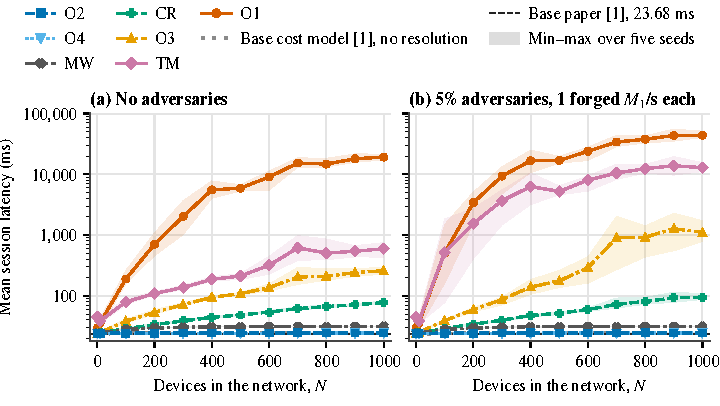
\includegraphics[width=\textwidth]{figs/fig_latency.pdf}
\caption{Mean session latency against network size in the OMNeT++ model (log scale; band: minimum to maximum over five
seeds). (a) Without adversaries. (b) With 5\% adversaries, each sending one forged $M_1$ per second. Dotted: the cost model of~\cite{base} with no resolution. Dashed: the base paper's 23.68\,ms.}
\label{fig:latency}
\end{figure*}

\subsection{Ranking}
\tabref{tab:ranked} gives the ranking. The two table strategies, O2 and O4, stay within 1\,ms of the base paper's figure up
to 1{,}000 devices. O2 needs one probe to slide the window, and O4 only the per-epoch extension. Their cost is memory: at
1{,}000 devices, about 93\,KiB and 46\,KiB per server, against 10\,KiB for Table~VI of~\cite{base} alone. The key tree is
third (31.4\,ms). It changes $M_1$, and a compromised device leaks the internal keys it shares with others. The
randomised hash lock (CR) needs no extra state, but its latency grows linearly, to 95\,ms. The three scanning strategies
with epochs saturate the server: clock scan (O3) at 1.1\,s, the time-memory trade-off at 12.9\,s, and the counter scan
(O1) at 44\,s. For O1 and TM, the spread across seeds at $N=1{,}000$ is 10.6\,s and 4.5\,s, because the latency depends on
how many devices and adversaries share the busiest server.

\subsection{Honest Load Against Forged Load}\label{sec:probes}
\figref{fig:latency} separates the two causes. Without adversaries (a), O1 already reaches 19.2\,s at 1{,}000 devices.
Each honest authentication costs about $12.5\,n$ probes, which is 1.0\,s of hashing at the $n\approx258$ devices that a
server enrols at $N=1{,}000$ ($T_H=0.32$\,ms). Arrivals outpace this, so the server queue grows. The forged load (b)
roughly doubles this, because every forged pseudonym costs a full miss scan of $Wn$ probes. Such a pseudonym never resolves
to a device, so the block-list, which blocks a device after three consecutive failed attempts, never sees it.
\figref{fig:probes} shows the same effect for one server enrolling up to $n=10{,}000$ devices. A forgery costs O1 250,000
probes and TM about 46,000, but costs O2 and O4 nothing, because a table miss needs no hash.

\floatstart{figure*}
\centering
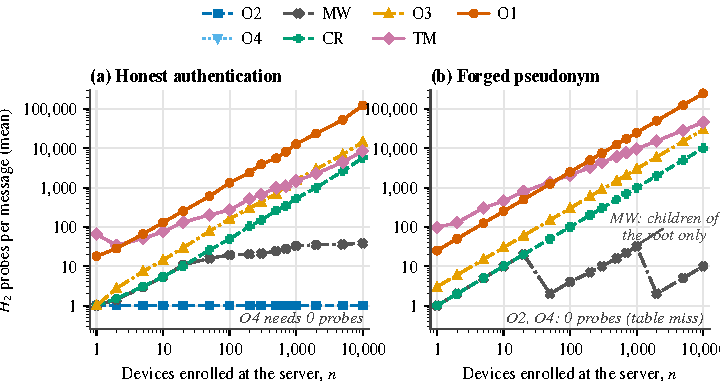
\includegraphics[width=\textwidth]{figs/fig_probes.pdf}
\caption{Probes per message at one server, measured on the implementation (log-log). (a) Honest authentication. (b) A
forged, random pseudonym.}
\label{fig:probes}
\end{figure*}

\subsection{Time Against Memory}
\figref{fig:storage} shows storage at one server, and each strategy's position in the time-memory plane for one server
enrolling $n=1{,}000$ devices. Storage is the resolution state plus the 40 bytes (320 bits) per device of Table~VI
of~\cite{base}. No strategy that keeps the wire format is both fast and small. O2 buys constant time with $F$ table entries
per device (359\,KiB in total), and O4 with $\Wc$ entries per device (180\,KiB). TM sits in between, at 167\,KiB and 1{,}478
probes. It is dominated here because its table must cover the device's whole lifetime ($m=128$ epochs), not just the
current window. MW is the only point that is both small and fast, and it pays with a different $M_1$ and a weaker privacy
model.

\floatstart{figure*}
\centering
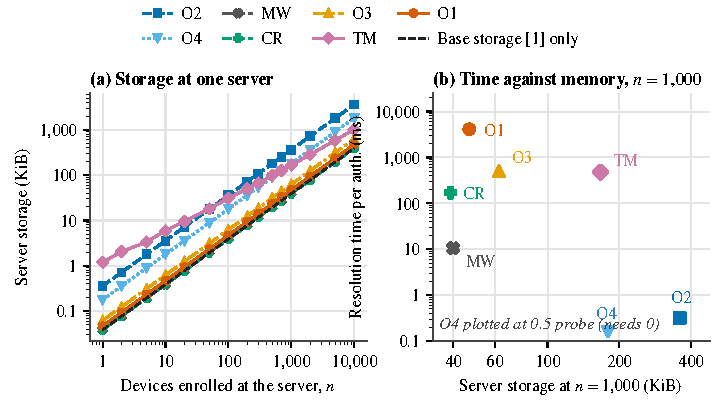
\includegraphics[width=\textwidth]{figs/fig_storage.pdf}
\caption{(a) Server storage (the 320 bits per device of Table~VI of~\cite{base} plus the resolution state) for one server.
(b) Resolution time per authentication ($T_H=0.32$\,ms per probe) against storage, for one server enrolling 1{,}000
devices.}
\label{fig:storage}
\end{figure*}

\subsection{Desynchronisation}\label{sec:desync}
With counter epochs, the device advances $t$ every time it builds $M_1$. The server searches at most $F$ epochs ahead of
the last one it accepted. In our implementation, an adversary who drops $F=8$ consecutive $M_1$ messages locks the device
out for good: every later handshake fails with an unknown pseudonym, with or without an earlier successful session. The
lockout holds for O1 and O2, and a unit test checks it for both. The threshold is $F$, which the specification does not
fix. A larger $F$ delays the lockout but does not remove it. A device whose counter lives in RAM is also rejected as
a replay after a restart; we observed this for O1. Message dropping is within the threat model of~\cite{base}. Clock epochs
(O3, O4), CR and MW have no per-device counter, so they cannot desynchronise this way. TM tolerates any number of drops
until $t$ reaches the lifetime $m$.

\subsection{Sensitivity to the Assumptions}\label{sec:sens}
The base paper does not fix the adversary share and rate, the authentication window or the enrolment rule, and $T_H$ is its
constant, not our measurement. We bound their effect without new simulation runs. First, the simulation was run with and
without adversaries (\figref{fig:latency}): at $N=1{,}000$ the ranking is the same, and O2, O4 and MW move by less than
0.2\,ms. Second, we compute the offered load of the mean server at $N=1{,}000$ from the committed cost model,
$\rho=\alpha_h(C_R+hT_H)+\alpha_a fT_H$, where $C_R=11.84$\,ms is the server cost per session from Tables~III and~V of~\cite{base},
$h$ and $f$ are the measured honest and forged probes at the mean enrolment $n=258$, and $\alpha_h$ and $\alpha_a$ are the
honest and forged arrival rates per server. $\rho\ge1$ means saturation (\tabref{tab:sens}).

\floatstart{table}
\centering
\caption{Offered load $\rho$ of the mean server at $N=1{,}000$, one assumption varied at a time from the baseline (5\%
adversaries at 1\,Hz, 10\,s window, reachable enrolment, $T_H=0.32$\,ms). $\rho\ge1$: saturated.}
\label{tab:sens}
\footnotesize
\setlength{\tabcolsep}{2.6pt}
\begin{tabular}{@{}l r r r r r r r@{}}
\toprule
Case & O2 & O4 & MW & CR & O3 & TM & O1 \\
\midrule
Baseline              & 0.02 & 0.03 & 0.04 & 0.19 & 0.52 & 1.68 & 4.16 \\
No adversaries        & 0.02 & 0.03 & 0.04 & 0.11 & 0.27 & 0.41 & 2.09 \\
20\% adversaries      & 0.02 & 0.03 & 0.05 & 0.44 & 1.26 & 5.47 & 10.3 \\
Adversary rate 2\,Hz  & 0.02 & 0.03 & 0.04 & 0.27 & 0.77 & 2.94 & 6.22 \\
Window 5\,s           & 0.05 & 0.06 & 0.08 & 0.30 & 0.79 & 2.09 & 6.25 \\
Window 20\,s          & 0.01 & 0.02 & 0.02 & 0.14 & 0.38 & 1.47 & 3.11 \\
$T_H=0.16$\,ms        & 0.02 & 0.03 & 0.03 & 0.11 & 0.27 & 0.85 & 2.09 \\
$T_H=0.64$\,ms        & 0.03 & 0.04 & 0.06 & 0.36 & 1.01 & 3.33 & 8.29 \\
Nearest enrolment     & 0.02 & 0.02 & 0.04 & 0.04 & 0.06 & 0.36 & 0.35 \\
\bottomrule
\end{tabular}
\end{table}

Except in the last row, the order by $\rho$ is that of \tabref{tab:ranked}, and O2 and O4 do not exceed 0.06. The
absolute figures do depend on the assumptions: O1 saturates unless $T_H<0.076$\,ms, and O3 saturates with 20\%
adversaries or $T_H=0.64$\,ms. (The busiest server enrols up to 396 devices, which is why O3 already queues in the
simulation at $\rho=0.52$.) If a server enrols only the devices attached to it ($n\approx20$), nothing saturates and the
lower ranks reorder, but O2 and O4 stay first. $L$, $F$ and $\Wc$ act only through the closed forms of
\designref. The recommendation of \secref{sec:disc} therefore holds under every assumption we varied, while
figures such as O1's 44\,s hold only under the baseline.

\iffv
\section{Formal Verification}\label{sec:fv}
We modelled the exchange in ProVerif~2.05~\cite{proverif}, in the symbolic model with an active attacker
(\tabref{tab:fv}). Other lightweight IoT schemes are checked in the same tool~\cite{wu22,lee25}; the scheme of~\cite{lee25},
for example, proves the privacy of its pseudonyms in ProVerif~2.05. Our hash, KDF and AEAD are free functions, and AEAD has
associated data. The main model has unbounded servers, unbounded honest and corrupt devices per server, and unbounded
sessions. A corrupt device's $\lambda$ and $k^\star$ are given to the attacker. The server may resolve a pseudonym to
\emph{any} enrolled device, and must then decrypt and check $\PID=H_2(\lambda_V\|t)$. So every result that holds, holds for
every resolver that returns a correct device. Epochs are fresh values, and the server keeps no replay state. Unlinkability
is checked as observational equivalence~\cite{blanchet08}, in the style of~\cite{arapinis}: one device running twice,
against two devices running once each. On both sides the server knows both devices and resolves with one destructor.

\floatstart{table}
\centering
\caption{ProVerif results (all models finish in under 1\,s).}
\label{tab:fv}
\footnotesize
\begin{tabular}{@{}l p{3.6cm} p{2.6cm}@{}}
\toprule
Query & Property & Result \\
\midrule
Q1, Q2 & Session key secret (device and server side) & holds \\
Q3 & Server accepts $M_1$ of honest $V$ $\Rightarrow$ $V$ sent it & holds \\
Q4 & Same, injective & fails (replay, no replay state) \\
Q5 & Device accepts $M_2$ $\Rightarrow$ server derived the same key, injective & holds \\
FS & Forward secrecy: key secret after later leak of $k^\star$ & fails (leak reveals the nonces) \\
U1 & Unlinkability, counter epochs & holds \\
U2 & Unlinkability, clock epochs, same epoch & fails (equal $\PID$s) \\
\bottomrule
\end{tabular}
\end{table}

These results separate the properties that the resolver cannot affect from those it decides:
\begin{itemize}
\item \emph{Independent of the resolver}: secrecy of the session key (Q1, Q2), agreement on $(V,R,N_i,t)$ (Q3), and
injective key agreement for the device (Q5). Q5 holds because $N_i$ is fresh and bound as associated data of $M_2$.
\item \emph{Decided by the epoch and replay choices}: injective authentication of the device (Q4) fails without replay
state. ProVerif finds a trace in which one $M_1$ is accepted twice. Injectivity therefore rests on the epoch window (O1,
O2, TM) or the nonce cache (O3, O4), which the specification leaves open. Tamarin analyses of EDHOC likewise find that not
all of its methods satisfy injective agreement~\cite{norrman21}. With clock epochs, the attacker links two sessions in one
epoch by testing their pseudonyms for equality (U2), a case of the tracking that TrackDev~\cite{budykho} formalises. With
counter epochs, the equivalence holds (U1).
\item \emph{Forward secrecy (FS)}: it does not hold, and the base paper does not claim it. A later leak of $k^\star$
reveals $N_i$, $N_j$ and $t$ from the ciphertexts, and with them the session key.
\end{itemize}

Q4 cannot be settled in ProVerif with the replay window included, because the window is mutable state. We check the
window by test instead, and leave a stateful proof (for example in Tamarin, as done for EDHOC~\cite{norrman23}) to future
work.
\fi

\section{Discussion}\label{sec:disc}
\runin{Deployment recommendation.} A server that uses counter epochs should precompute (O2). One probe per
authentication and no hashing on forged input remove both the scaling and the denial-of-service problem, at about
$40F$ bytes per device. The lockout after $F$ dropped messages remains, so the device needs a resynchronisation path, or
the server needs a larger $F$, which costs table space linearly. If devices have clocks, O4 is faster than O2 up to 500
devices in \tabref{tab:ranked} and needs half the memory of O2, although O2 is faster at 1{,}000 devices (24.40\,ms against
24.59\,ms). O4 makes sessions within one epoch linkable and needs a nonce cache for replay detection. The epoch length then
trades privacy against the per-epoch rebuild of $n$ probes. On-demand scanning (O1, O3) is acceptable only for small $n$
and a trusted network. With 5\% adversaries, O1 is already 21 times the base paper's per-session cost at 100 devices.

\ifshortpaper\else
\runin{Specification gaps.} The protocol needs three decisions that it does not state: the epoch
semantics, the resolution method, and the replay state that makes device authentication injective. Its cost model
needs a resolution term. That term is $(n-1)W/2+L+2$ probes for an on-demand counter scan, and at least one probe or
one table lookup for a precomputed table. Its storage model needs the table.
\fi

\section{Limitations}\label{sec:lim}
\begin{itemize}
\item The simulation is our model of the environment of the base paper; the model of its authors is not available. Our
adversary, window and enrolment assumptions set the saturated latencies of O1, O3 and TM but not the lead of O2 and O4;
beyond the adversary share, this is shown from the mean-server load, not new runs (\secref{sec:sens}).
\item We price probes with the constant of Table~III of~\cite{base} ($T_H=0.32$\,ms) and report no hardware timings.
\item CR and MW change $M_1$ and are modelled at the resolution level only. The TM parameters (six tables, $m=128$) are
one point of its trade-off curve.
\item Our epoch, window and table choices are ours, and conformance means agreement with our reading of Section~III
of~\cite{base}, which only its authors can confirm.
\iffv
\item The ProVerif results are symbolic and assume perfect primitives.
\else
\item We give no formal proof.
\fi
\end{itemize}

\section{Conclusion}\label{sec:concl}
We set out to determine how the unspecified resolution step of~\cite{base} can be filled and what the choice decides.
(i)~\emph{Requirement.} Every correct server must resolve the pseudonym before any cryptographic check. The specification
leaves open the epoch semantics, the resolution method and the replay state, and its cost model has no term for the step.
(ii)~\emph{Cost.} Under the base paper's own constants and network, the choice decides whether a session stays at its
23.68\,ms or reaches tens of seconds at 1{,}000 devices. Precomputed tables (O2, O4), the oldest answer from RFID private
identification, stay within 1\,ms of the published figure at 46--93\,KiB per server. The lead of O2 and O4 holds under every
assumption we varied, while the size of the slowdown depends on them.
(iii)~\emph{Failure modes.} With on-demand scanning, every forged pseudonym costs a full scan that the block-list never
sees, while a table rejects it with no hashing. Counter epochs lock a device out after $F$ dropped messages, so a
deployment needs a resynchronisation path.
\iffv
(iv)~\emph{Security.} Session-key secrecy and agreement do not depend on the resolver, while unlinkability and injective
device authentication depend on the epoch and replay choices.
\fi
\ifanonymous
The implementation, the counting scripts, the OMNeT++ model\iffv, the ProVerif models\fi{} and all results are open in
the repository (link withheld for anonymous review).
\else
The implementation, the counting scripts, the OMNeT++ model\iffv, the ProVerif models\fi{} and all results are open at
\url{https://github.com/jaykerkar0405/hybrid-ecc-iot-auth}.
\fi

\ifbibtexrefs
\ifanonymous\else
\begin{credits}
\subsubsection{\ackname} This work was carried out as part of the Capstone Project course during semesters 6 and 7 at
Vivekanand Education Society's Institute of Technology. No funding was received for this research.
\subsubsection{\discintname} The Capstone Project course requires students to protect their work by a patent, copyright or
trademark filing before publishing it. The authors have no other competing interests to declare.
\end{credits}
\fi
\bibliographystyle{splncs04}
\bibliography{../refs}
\else
\begin{thebibliography}{99}
\bibitem{base} A. Al-Rasheed, R. Khan, A. Ahmad, A. Saeed, F. Alturise, and S. Alkhalaf, ``A low-cost hybrid elliptic curve cryptography authentication protocol for trustworthy Internet of Things communication,'' \emph{IEEE Trans. Consum. Electron.}, vol.~72, no.~2, pp.~4483--4491, May 2026, \doi{10.1109/TCE.2026.3662053}
\bibitem{weis} S. A. Weis, S. E. Sarma, R. L. Rivest, and D. W. Engels, ``Security and privacy aspects of low-cost radio frequency identification systems,'' in \emph{Security in Pervasive Computing (SPC 2003)}, ser. Lecture Notes in Computer Science, vol.~2802. Springer, 2004, pp.~201--212, \doi{10.1007/978-3-540-39881-3_18}
\bibitem{ohkubo} M. Ohkubo, K. Suzuki, and S. Kinoshita, ``Cryptographic approach to `privacy-friendly' tags,'' in \emph{RFID Privacy Workshop}, MIT, Cambridge, MA, USA, Nov. 2003.
\bibitem{molnar} D. Molnar and D. Wagner, ``Privacy and security in library RFID: Issues, practices, and architectures,'' in \emph{Proc. 11th ACM Conf. Comput. Commun. Secur. (CCS)}, Oct. 2004, pp.~210--219, \doi{10.1145/1030083.1030112}
\bibitem{avoine05} G. Avoine and P. Oechslin, ``A scalable and provably secure hash-based RFID protocol,'' in \emph{Proc. 3rd IEEE Int. Conf. Pervasive Comput. Commun. Workshops (PerCom Workshops)}, 2005, pp.~110--114, \doi{10.1109/PERCOMW.2005.12}
\bibitem{ado05} G. Avoine, E. Dysli, and P. Oechslin, ``Reducing time complexity in RFID systems,'' in \emph{Selected Areas in Cryptography (SAC 2005)}, ser. Lecture Notes in Computer Science, vol.~3897. Springer, 2006, pp.~291--306, \doi{10.1007/11693383_20}
\bibitem{tsudik} G. Tsudik, ``YA-TRAP: Yet another trivial RFID authentication protocol,'' in \emph{Proc. 4th IEEE Int. Conf. Pervasive Comput. Commun. Workshops (PerCom Workshops)}, 2006, pp.~640--643, \doi{10.1109/PERCOMW.2006.152}
\bibitem{tiplea} F. L. \c{T}iplea and C. Hristea, ``Practically efficient RFID scheme with constant-time identification,'' in \emph{Proc. 18th Int. Conf. Secur. Cryptogr. (SECRYPT)}. SciTePress, 2021, pp.~495--506, \doi{10.5220/0010544804950506}
\bibitem{gcm} M. Dworkin, ``Recommendation for block cipher modes of operation: Galois/Counter Mode (GCM) and GMAC,'' NIST, NIST SP 800-38D, Nov. 2007, \doi{10.6028/NIST.SP.800-38D}
\bibitem{hkdf} H. Krawczyk and P. Eronen, ``HMAC-based extract-and-expand key derivation function (HKDF),'' IETF, RFC 5869, May 2010, \doi{10.17487/RFC5869}
\bibitem{fips180} National Institute of Standards and Technology, ``Secure hash standard (SHS),'' NIST, FIPS PUB 180-4, Aug. 2015, \doi{10.6028/NIST.FIPS.180-4}
\bibitem{hellman} M. E. Hellman, ``A cryptanalytic time-memory trade-off,'' \emph{IEEE Trans. Inf. Theory}, vol.~26, no.~4, pp.~401--406, Jul. 1980, \doi{10.1109/TIT.1980.1056220}
\bibitem{oechslin} P. Oechslin, ``Making a faster cryptanalytic time-memory trade-off,'' in \emph{Advances in Cryptology -- CRYPTO 2003}, ser. Lecture Notes in Computer Science, vol.~2729. Springer, 2003, pp.~617--630, \doi{10.1007/978-3-540-45146-4_36}
\bibitem{omnet} A. Varga and R. Hornig, ``An overview of the OMNeT++ simulation environment,'' in \emph{Proc. 1st Int. ICST Conf. Simul. Tools Techn. Commun. Netw. Syst. (SIMUTools)}. ICST, 2008, \doi{10.4108/ICST.SIMUTOOLS2008.3027}
\iffv
\bibitem{proverif} B. Blanchet, ``Modeling and verifying security protocols with the applied pi calculus and ProVerif,'' \emph{Found. Trends Privacy Secur.}, vol.~1, no.~1--2, pp.~1--135, Oct. 2016, \doi{10.1561/3300000004}
\bibitem{wu22} T.-Y. Wu, Q. Meng, S. Kumari, and P. Zhang, ``Rotating behind security: A lightweight authentication protocol based on IoT-enabled cloud computing environments,'' \emph{Sensors}, vol.~22, no.~10, Art. no.~3858, May 2022, \doi{10.3390/s22103858}
\bibitem{lee25} H. J. Lee, S. Kook, K. Kim, J. Ryu, Y. Lee, and D. Won, ``LAMT: Lightweight and anonymous authentication scheme for medical Internet of Things services,'' \emph{Sensors}, vol.~25, no.~3, Art. no.~821, Jan. 2025, \doi{10.3390/s25030821}
\bibitem{blanchet08} B. Blanchet, M. Abadi, and C. Fournet, ``Automated verification of selected equivalences for security protocols,'' \emph{J. Log. Algebr. Program.}, vol.~75, no.~1, pp.~3--51, Feb. 2008, \doi{10.1016/j.jlap.2007.06.002}
\bibitem{arapinis} M. Arapinis, T. Chothia, E. Ritter, and M. Ryan, ``Analysing unlinkability and anonymity using the applied pi calculus,'' in \emph{Proc. 23rd IEEE Comput. Secur. Found. Symp. (CSF)}, Jul. 2010, pp.~107--121, \doi{10.1109/CSF.2010.15}
\bibitem{norrman21} K. Norrman, V. Sundararajan, and A. Bruni, ``Formal analysis of EDHOC key establishment for constrained IoT devices,'' in \emph{Proc. 18th Int. Conf. Secur. Cryptogr. (SECRYPT)}. SciTePress, 2021, pp.~210--221, \doi{10.5220/0010554002100221}
\bibitem{budykho} K. Budykho \emph{et al.}, ``Fine-grained trackability in protocol executions,'' in \emph{Proc. Netw. Distrib. Syst. Secur. Symp. (NDSS)}. Internet Society, 2023, \doi{10.14722/ndss.2023.24289}
\bibitem{norrman23} K. Norrman, V. Sundararajan, and A. Bruni, ``Extended formal analysis of the EDHOC protocol in Tamarin,'' in \emph{E-Business and Telecommunications}, ser. Communications in Computer and Information Science. Springer, 2023, pp.~224--248, \doi{10.1007/978-3-031-36840-0_11}
\fi
\end{thebibliography}
\fi

\end{document}
